\chapter{Feasibility study of discrete symmetry violation searches with the J-PET detector}
\label{chapter:analysis_jpet}

The J-PET detector aims at recording a large sample of ortho-positronium decays into three photons in order to measure the expectation values of several angular correlation operators odd under the \Ts, \CPs~and \CPTs~symmetries (see~\tref{tab:jpet_operators}). Each of these operator involves spin of the decaying \ops/, which, however, cannot be measured directly in the experiment.
While previous studies of \ops/$\to 3\gamma$ decays used strong external magnetic field~\cite{cp_positronium} or~limited the momenta of positrons creating \ops/ atoms to a hemisphere and incorporated the further positronium polarization into systematic uncertainty~\cite{cpt_positronium}, a different approach was proposed by the J-PET experiment.
Alike the latter of aforementioned experiments, J-PET will estimate spin directions of ortho-positronium atoms using momentum of the original positrons. However, the latter may be reconstructed separately for each recorded event of \ops/ decay using the procedure presented in~\sref{sec:ops_polarization}.

The key requirements to implement this measurement scheme comprise:
\begin{itemize}
\item the possibility to identify \ops/$\to 3\gamma$ events among recorded background,
\item reconstructing the decay points inside the \ops/ production medium,
\end{itemize}
where achievable resolution of such reconstruction will dictate the level of precision at which the positronium spin polarization is controlled.

\section{Resolution tests with Monte Carlo Simulations}
\label{sec:jpet_mc_tests}
First tests of the the ortho-positronium decay reconstruction were performed with dedicated Monte Carlo simulations
of \ops/$\to 3\gamma$ decays recorded by a detection setup similar to J-PET. 
Prior to positronium annihilations, the simulation involved emission of positrons from a $^{22}$Na $\beta^+$ source and their thermalization in a porous medium with a possibility to form an \ops/ atom. The detector implemented in the simulation was built of plastic scintillator strips with the same properties as J-PET (compare~\sref{sec:jpet}) but had an idealized geometrical acceptance obtained with four concentric cylindrical layers of detection modules mounted without gaps between them. Further details of the simulated setup can be found in Reference~\cite{gajos_gps}.

Like in the J-PET detector, photon interaction point in a scintillator was resolved in the simulation up to the strip location, resulting in a precision of about 0.5$^{\circ}$. The assumed resolutions of longitudinal ($z$) $\gamma$ interaction position and its time were varied in order to explore the sensitivity of the reconstruction to uncertainty of each input parameter. For a number of $10^{5}$ of simulated and fully recorded \ops/$\to 3\gamma$ events, their simulated origins were compared to the decay points reconstructed with the technique presented in~\cref{chapter:gps}. For each of the Cartesian coordinates, the $\sigma$ value of the resulting distributions of simulated-reconstructed discrepancies was used as an estimate of spatial resolution.

\begin{figure}[h!]
  \centering
  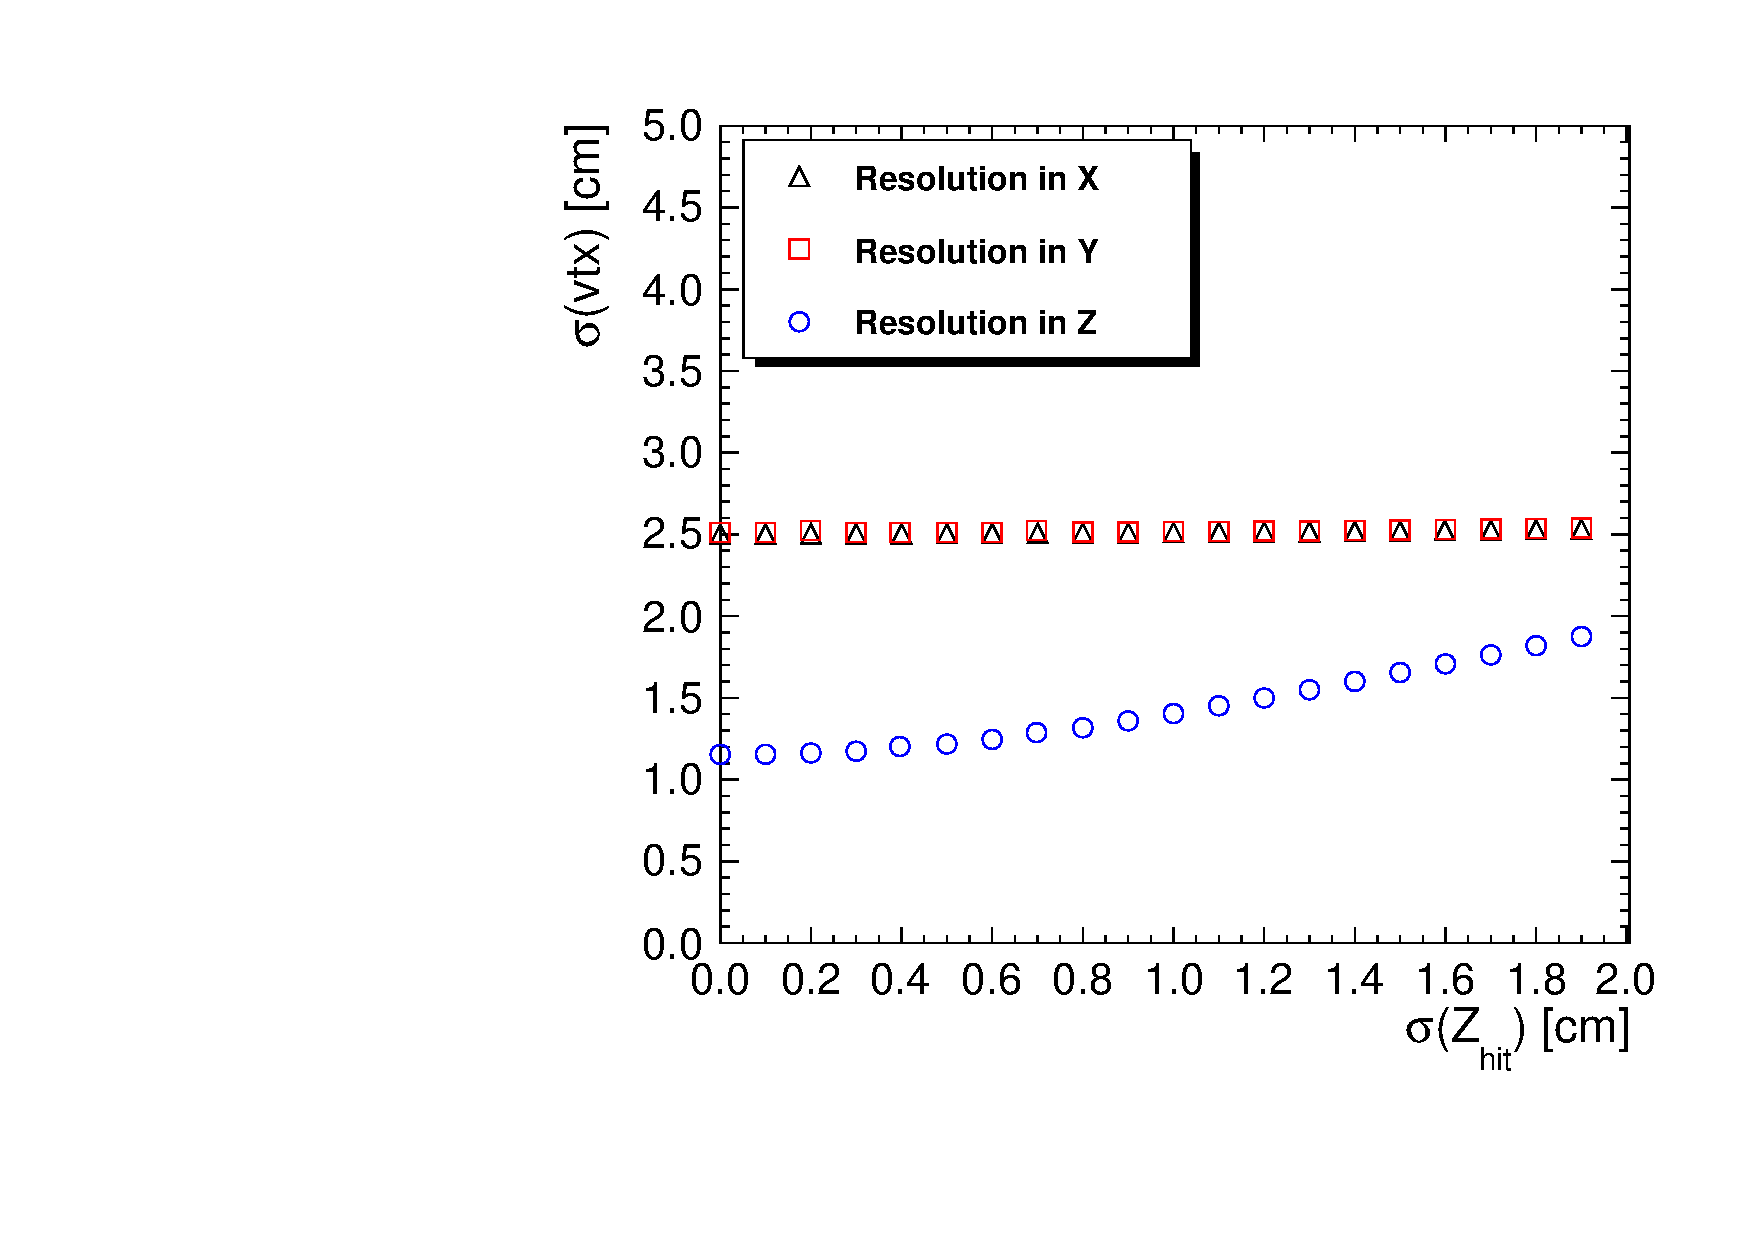
\includegraphics[width=0.45\textwidth]{Chapter8_analysis_jpet/img/res_vs_z}
  \hspace{1em}
  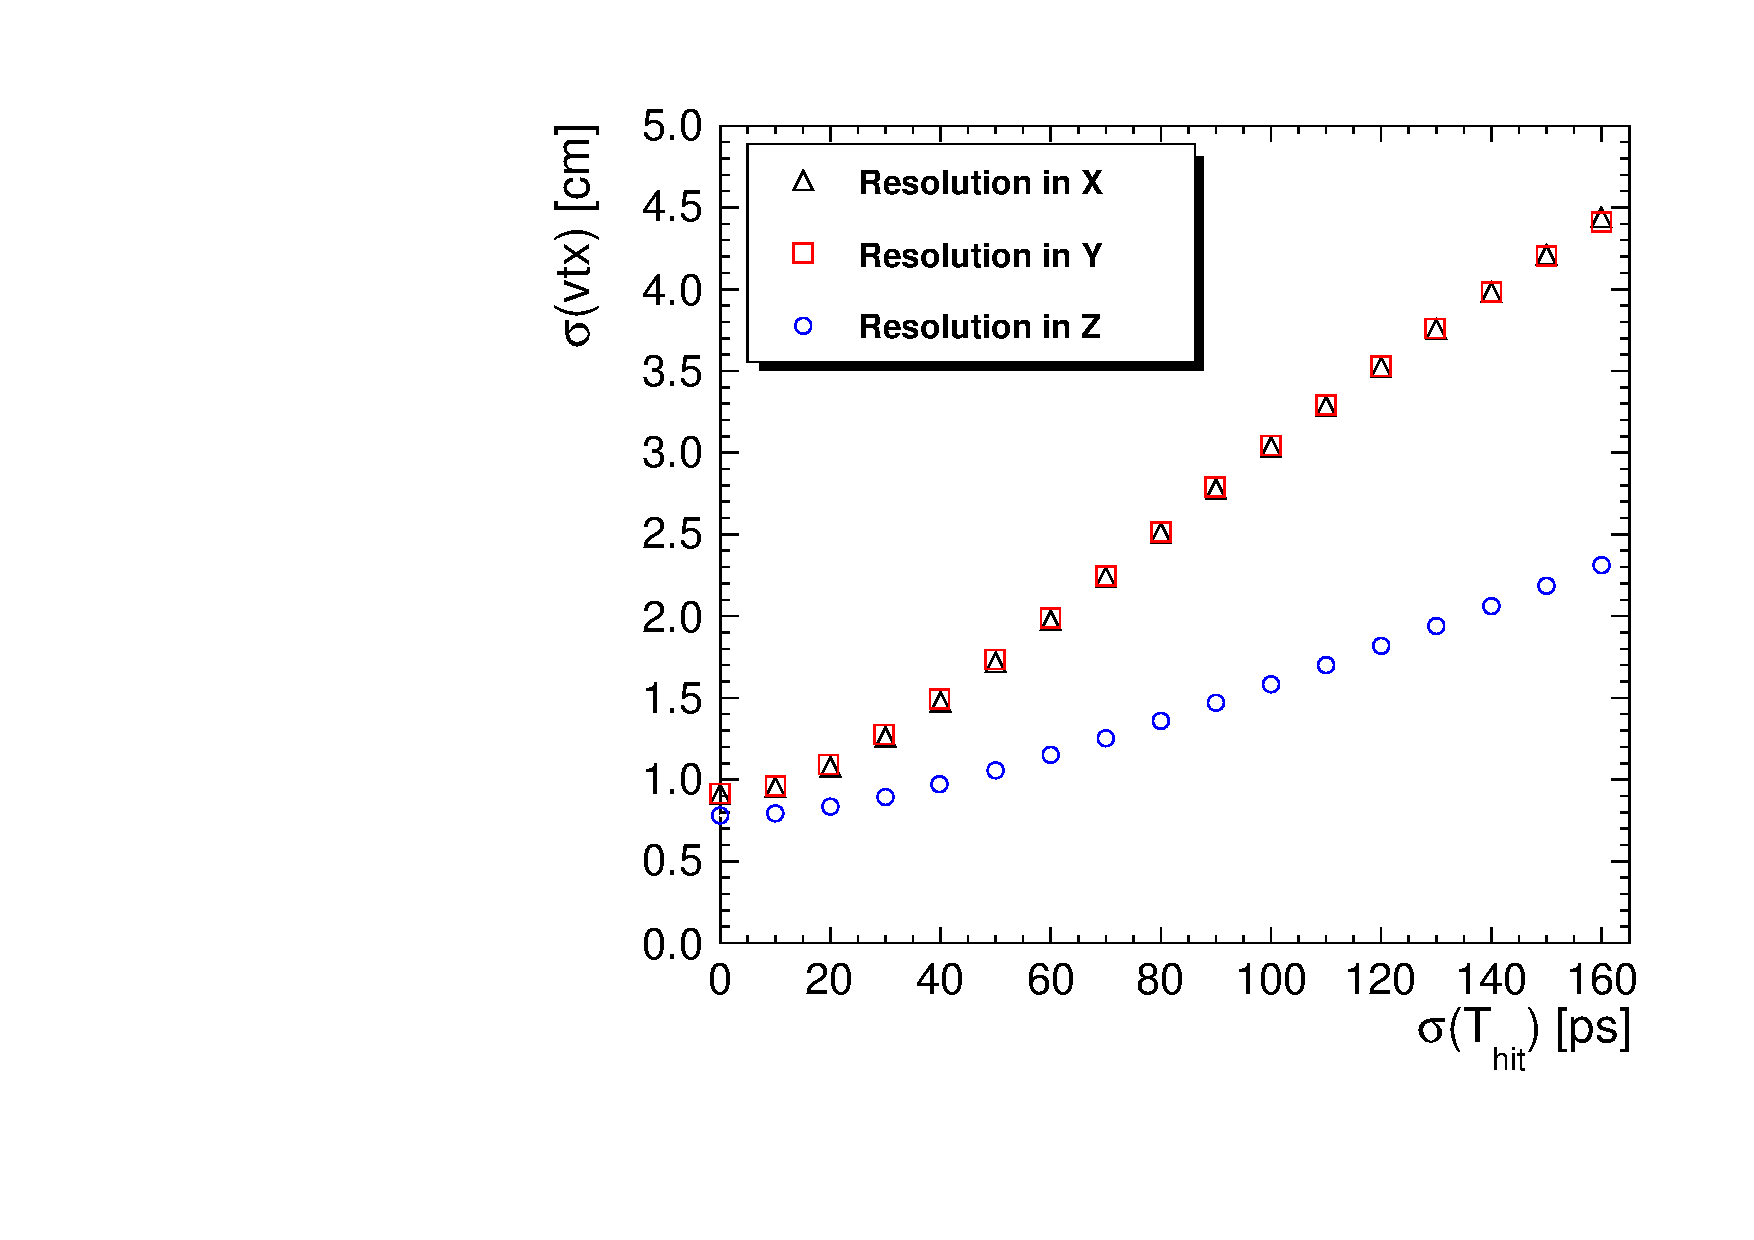
\includegraphics[width=0.45\textwidth]{Chapter8_analysis_jpet/img/res_vs_t}
  \caption{Spatial resolution of Cartesian coordinates of the \ops/$\to 3\gamma$ decay point as a function of the detector resolution of $\gamma$ interactions in the scintillator strips, in terms of the interaction longitudinal position (left) and interaction time (right). Figures adapted from~\cite{gajos_gps}.}\label{fig:jpet_mc_res}
\end{figure}

\fref{fig:jpet_mc_res} presents the obtained distributions of the resolution depending on the accuracy of $\gamma$ interaction properties recorded by the detector. As visible in the right panel, the tested reconstruction method exhibits largest sensitivity to temporal resolution.
%
At the same time, the impact of $z$ coordinate determination for photon interactions in scintillator strips is only visible in the decay point resolution along the $z$ axis, distinguished by the cylindrical geometry of the detector as well as a different resolution than in the transverse plane.
%
The pronounced sensitivity of reconstruction to time of recorded photon interactions with respect to their $z$-coordinate resolutions is caused by the fact that while $\sigma(t_{\gamma})$ and $\sigma(z_{\gamma})$ are connected approximately by a factor equal to the effective velocity of light in a scintillator strip ($\upsilon_{eff}\approx 12\:\frac{\text{cm}}{\text{ns}}$), the errors on time determination propagate to the final result multiplied by the velocity of light in vacuum (see~\aref{appendix:jpet_solution}), larger by a factor of~2.5.
%
% TODO: dopisać o kątowej rozdzielczości i jej wpływie na polaryzację
%

The demonstrated sensitivity of this reconstruction technique to errors of photon recording times may, however, be turned into an advantage when this method is employed for background discrimination.
The positron source assumed in the MC simulations had an activity 10~MBq, of the same order as sources planned for J-PET measurements. This allowed to test the capability of the trilaterative reconstruction to reject background originating from accidental photon coincidences. As estimated in a separate study~\cite{kowalski_scatter_fraction}
the rate of such coincidences expected with the aforementioned source activity and a time window of 5~ns would be about 1/5 of the total rate. Monte Carlo simulations performed for such conditions yielded an accidental coincidence rate of 2800/s~\cite{gajos_gps}. Since in the accidental $3\gamma$ sets at least one of the quanta does not originate in the same decay as the other ones, event slight inconsistencies of the photons' creation times lead to the reconstructed annihilation point located either in a non-physical region or at a considerable distance from the \ops/ creation medium. Therefore, a requirement of the reconstructed point distance from the volume of possible positronium decays allowed to reduce the rate of accidental triple coincidences by a factor of \SI{89}{\percent} in the MC-based studies~\cite{gajos_gps}.

As discussed in~\sref{sec:ops_polarization}, the polarization along a given axis for positrons from a $\beta^+$ decay whose direction of momentum is known with an angular uncertainty described by a cone around this axis and an opening angle $\alpha$ is given by the relation:
\begin{equation}
  \label{eq:jpet_positron_polarization}
  P_{e+} = \frac{\upsilon_{e+}}{c}\frac{1+\cos(\alpha)}{2},
\end{equation}
where $\upsilon_{e+}$ is the average positron velocity and $c$ denotes the velocity of light~\cite{Coleman}. The level of average polarization of the \ops/ atoms inferred from the incident positrons hence depends on the angular resolution of $e^+$ momentum if a setup like the one presented in~\fref{fig:ops_spin_determination} is used. The tests with MC-simulated $3\gamma$ events originating in the wall of the cylindrical chamber have shown that, after inclusion of a kinematical fit restricting the reconstructed decay points in the transverse radius cylindrical coordinate to lie in the chamber material, the angular uncertainty of the positron motion direction can be reduced to about~\SI{15}{\degree}. It follows from~\eref{eq:jpet_positron_polarization} that
such event-wise estimation of the $e^+$ spin direction
allows to retain $\frac{1}{2}(1+\cos(15^{\circ}))\approx$\SI{98}{\percent} of the polarization resulting from parity violation in the $\beta$ decay~\cite{gajos_gps}.

\section{Analysis of first J-PET measurement with $3 \gamma$ annihilation medium}\label{sec:jpet_firs_data}

\subsection{The test experimental setup}
\label{sec:jpet_test_setup}
The first measurement with the J-PET detector implementing the scheme discussed in~\sref{sec:ops_polarization} was carried out with an aluminum vacuum chamber depicted in~\fref{fig:jpet-source} (left). The chamber was shaped as a cylinder with a diameter of about 14~cm. In the center of the chamber a $\beta^+$ source was placed in the form of $^{22}$Na enclosed by two layers of kapton foil spanned by a metal frame as presented in ~\fref{fig:jpet-source} (right). A vacuum system connected to the chamber ensured pressure at a level of about 8~mbar inside its volume.

\begin{figure}[h!]
  \centering
\begin{tikzpicture}[
  scale=0.5,
  >={Stealth[inset=0pt,length=6pt,angle'=50,round]}
  ]
  % dummy rect
  \draw[white] (-5.5,-6) rectangle (9,6);
  
  % detector
  \draw[fill=black!50!white] (-5,4.1) rectangle (5,4.3) node[right, yshift=-7] {\large Layer 1};
  \draw[fill=black!50!white] (-5,4.6) rectangle (5,4.8) node[right] {\large Layer 2};
  \draw[fill=black!50!white] (-5,5.6) rectangle (5,5.8) node[right] {\large Layer 3};

  \draw[fill=black!50!white] (-5,-4.3) rectangle (5,-4.1);
  \draw[fill=black!50!white] (-5,-4.8) rectangle (5,-4.6);
  \draw[fill=black!50!white] (-5,-5.8) rectangle (5,-5.6);
  
  \draw[line width=3pt, black!50!white] (-5,-0.65) -- (-5,0.65) -- (5,0.65) -- (5,0.2) -- (5.4, 0.2);
  \draw[line width=3pt, black!50!white] (-5,-0.65) -- (5,-0.65) -- (5,-0.2) -- (5.4, -0.2);
  \node[] at (6.8, 0) {\large $\rightarrow$ vacuum};
  \node[] at (7.2, -0.7) {\large system};
  
  \draw[line width=3pt, black] (0, -0.65) -- (0, -0.15);
  \draw[line width=3pt, black] (0, 0.65) -- (0, 0.15);
  \draw[line width=1pt, black] (0, 0.15) -- (0, -0.15);

  \draw[thick,<->] (2,-0.65) -- (2,0.65) node[midway, right] {\large 14~cm};

  \draw[black] (0.1, 0.3) -- (1.5, 2.0) -- (2.0, 2.0);
  \node[right] at (2.0, 2.0) {\large $\beta^+$ source holder};

  % max and min paths
  % \draw[darkgray, line width=1pt, dashed, ->] (-4.9,-0.65) -- (-4.9,-4.1);
  % \draw[darkgray, line width=1pt, dashed, ->] (-4.9,0.65) -- (4.9,-5.6);
  
\end{tikzpicture}
\hspace{1ex}
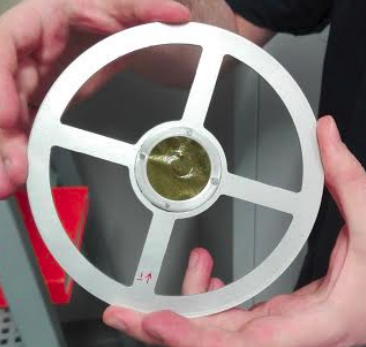
\includegraphics[width=0.40\textwidth]{Chapter8_analysis_jpet/img/source}
  \caption{Left: cross section view scheme of the setup used in the test measurement with a 3$\gamma$ event production chamber. Right: setup of the $^{22}$Na $\beta^+$ source mounted in the center of the $3\gamma$ production chamber. The source was enclosed between two layers of kapton foil spanned on an aluminum frame mounted to the inner walls of the chamber. The chamber and source were constructed at the Maria Curie-Sk\l{}odowska University by a subgroup of the J-PET collaboration.}\label{fig:jpet-source}
\end{figure}

As the porous aerogel material intended as a positronium creation medium was in preparation at the time of the test measurement, the chamber walls contained no additional material besides aluminum.
Although the probability of ortho-positronium formation in aluminum is negligibly low, direct electron-positron annihilation into three photons is possible and may be used to test the procedures for identification and reconstruction of such events regardless of the origin of the 3$\gamma$ state.

As the yield of 3$\gamma$ events from direct annihilation is smaller than the expected rate from decays of ortho-positronium produced in aerogel by a factor of about 400, a demonstration of the possibility to identify such events in the data of such test measurement would guarantee the feasibility of handling the \ops/$\to 3\gamma$ decays in the future experiments with J-PET\@.

\subsection{Data reconstruction and preselection}
\label{sec:jpet_preselection}
The test measurement was performed for two days, resulting in a total of 5.5~TB of collected raw data. Reduction of such a high data flux, resulting from the triggerless mode of J-PET data acquisition~\cite{greg_daq}, requires stringent discrimination of background in order to allow for effective analysis of the J-PET data. The analysis of the test data was performed using the J-PET Analysis Framework software~\cite{Krzemien:2015hkb}. At the first stages of data reconstruction, single times recorded at certain voltage thresholds applied to the PMT electric signals were assembled into representations of these signals as presented in~\fref{fig:jpet_signal}. For each signal, the time over threshold (TOT) value was calculated (see~\eref{eq:tot_i}) using information on all available thresholds. Subsequently, pairs of signals (referred to as \textit{hits} in the further considerations) coming from the same $\gamma$ interaction were identified. Signals were paired if they originated from distinct sides of the same detection module (scintillator strip) and their arrival times (estimated using time at the leading edge on a threshold lowest in terms of absolute voltage) were separated by no more than 5~ns. The last stage of early reconstruction comprised assembling event candidates as sets of hits contained within a time window of 20~ns. Although such a time window is broad with respect to possible time differences in a physical event, its purpose was a reduction of data volume without limiting further fine selection of event candidates by more strict timing requirements. Only event candidates with at least 3 hits within 20~ns were accepted for further analysis which allowed for reduction of the raw data by about \SI{98.8}{\percent}.

After preselection of event candidates described above, a total sum of times over threshold for both signals comprising each hit was calculated (see~\eref{eq:tot_def}) as a measure of the deposited energy of a corresponding $\gamma$ quantum. However, such estimation of the deposited energy through size of the electric signals is sensitive to effects of properties of the detector such as gain of the photomultipliers, which may vary between modules. Therefore, a simple calibration of the TOT values was performed. 

\subsection{Calibration of time over threshold (TOT) values}
\label{sec:jpet_tot_calib}
The TOT calibration was performed using a sample of direct $e^+e^-\to 2\gamma$ annihilation events for which the initial energy of the photons interacting in J-PET scintillators is well defined (511~keV). Such events were selected using criteria described in Reference~\cite{monika_2gamma_imaging}. For each of the 192 detection modules of J-PET, a separate distribution of the TOT$_{\gamma}$ values was obtained using hits from the selected two-photon annihilation events. In each spectrum, mode TOT$_{\gamma}$ value was identified as a weighted average of the centers of the most populated bin in the histogram and its neighboring bins. Thus obtained mode corresponds to the most probable deposited energy in a Compton spectrum for 511~keV photons, which amounts to about 280~keV.
In order to equalize the TOT responses of particular detection modules,
the following relation between TOT and deposited energy was used:
\begin{equation}
  \label{eq:tot_edep}
  E_{dep}(TOT_{\gamma}) \text{[keV]} = \exp\left( \left( TOT\text{[ps]} + 1.1483\times 10^{5} \right) / 23144  \right),
\end{equation}
which had been determined experimentally using J-PET data and an approach similar as discussed in Reference~\cite{tot_edep}. For each detection module $k$, a correction factor was calculated as a ratio of the most probable deposited energy to the time over threshold mode TOT$_{M}$ obtained for that module and transformed to deposited energy:
\begin{equation}
  \label{eq:tot_corr}
  \alpha_{k} = \frac{280\ \text{keV}}{E_{dep}(TOT^{(k)}_{M})}.
\end{equation}

Calibration factors obtained in this manner for each of the 192 scintillators of the detector were applied in the analysis of the test measurement with 3$\gamma$ production chamber. For every recorded hit, its calculated TOT value was transformed to deposited energy, multiplied by the correction factor relevant to the detection module in which it was recorded, and transformed back to time over threshold.
\begin{figure}[h!]
  \centering
  \begin{tikzpicture}
    \node[anchor=south west,inner sep=0] at (0,0) 
    {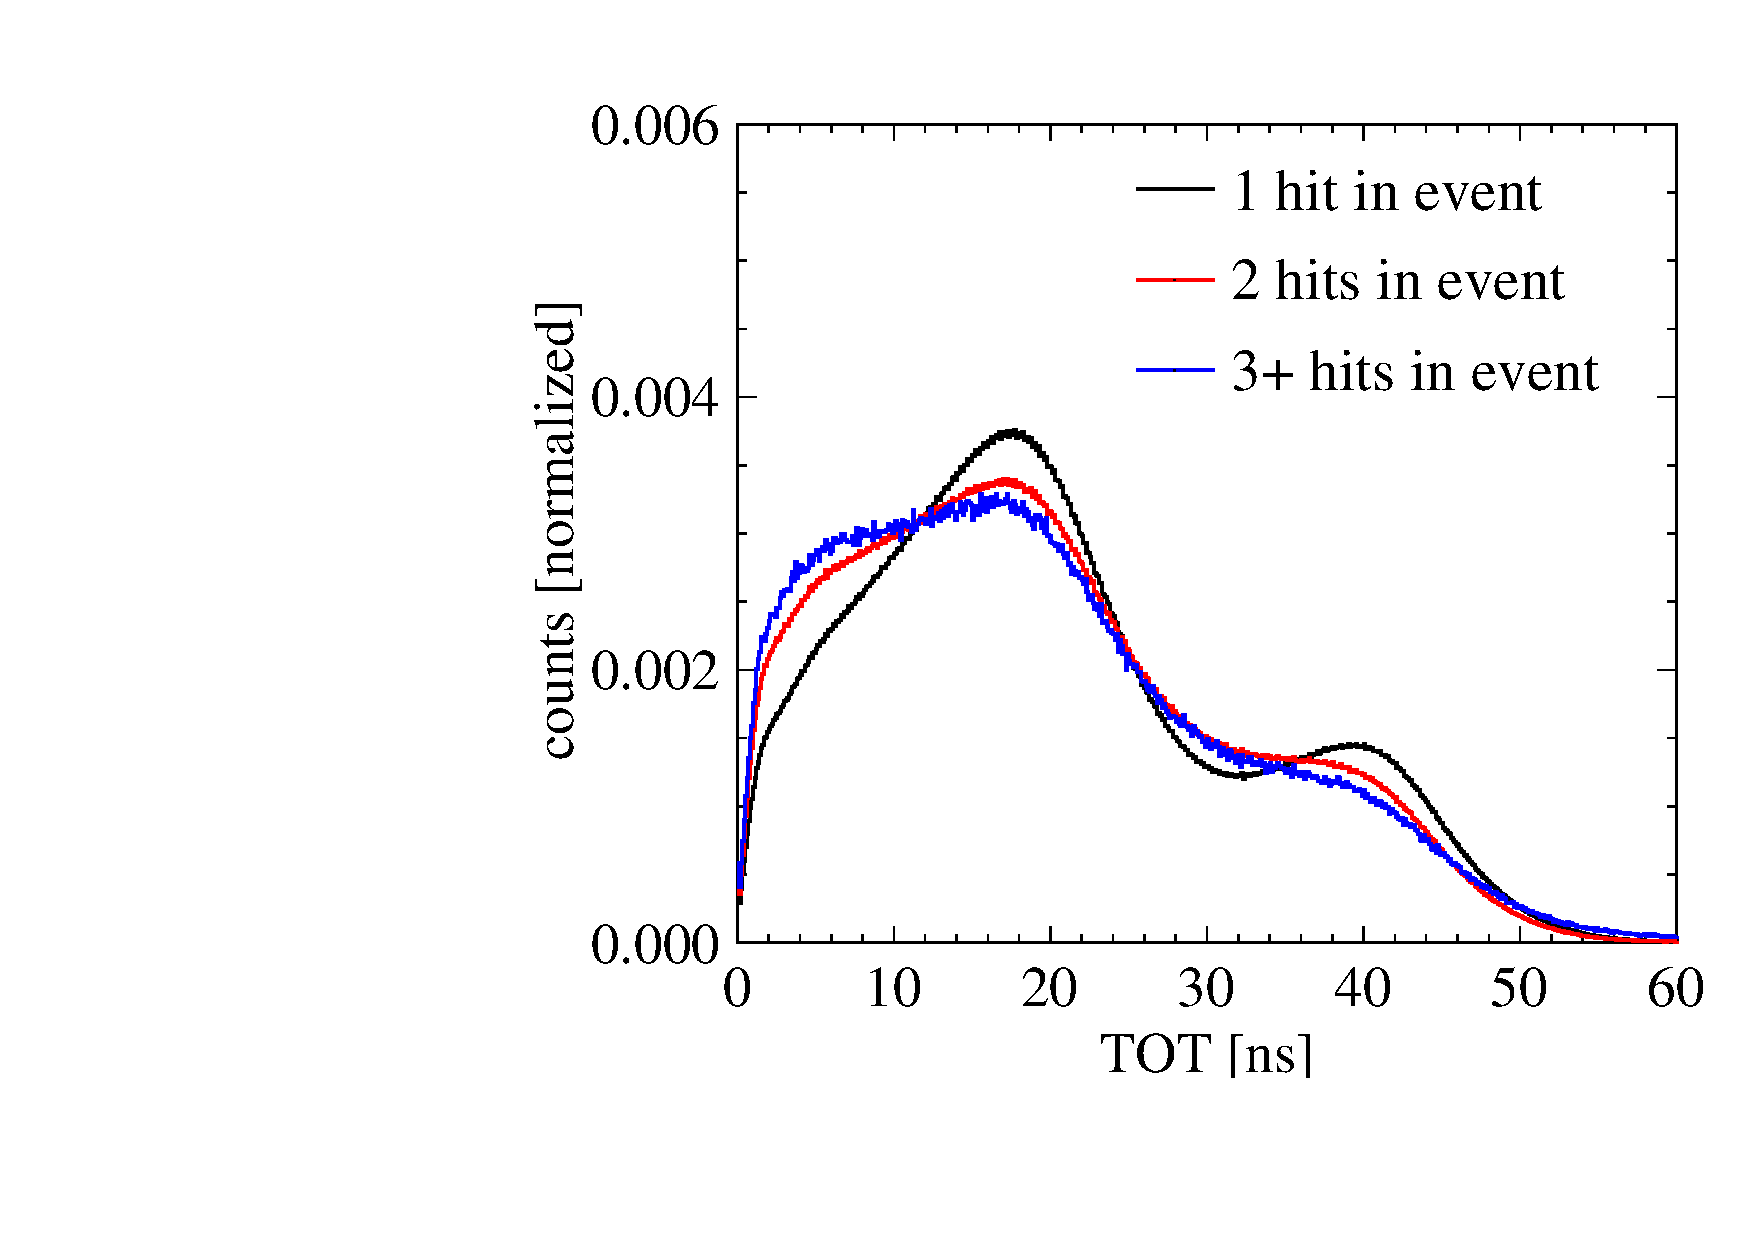
\includegraphics[width=0.45\textwidth]{Chapter8_analysis_jpet/img/tots_raw}};
%    \draw[black, thick, dashed] (2.50,5.0) -- (5.50,2.0);
  \end{tikzpicture}
  \hspace{1em}
    \begin{tikzpicture}
    \node[anchor=south west,inner sep=0] at (0,0) 
    {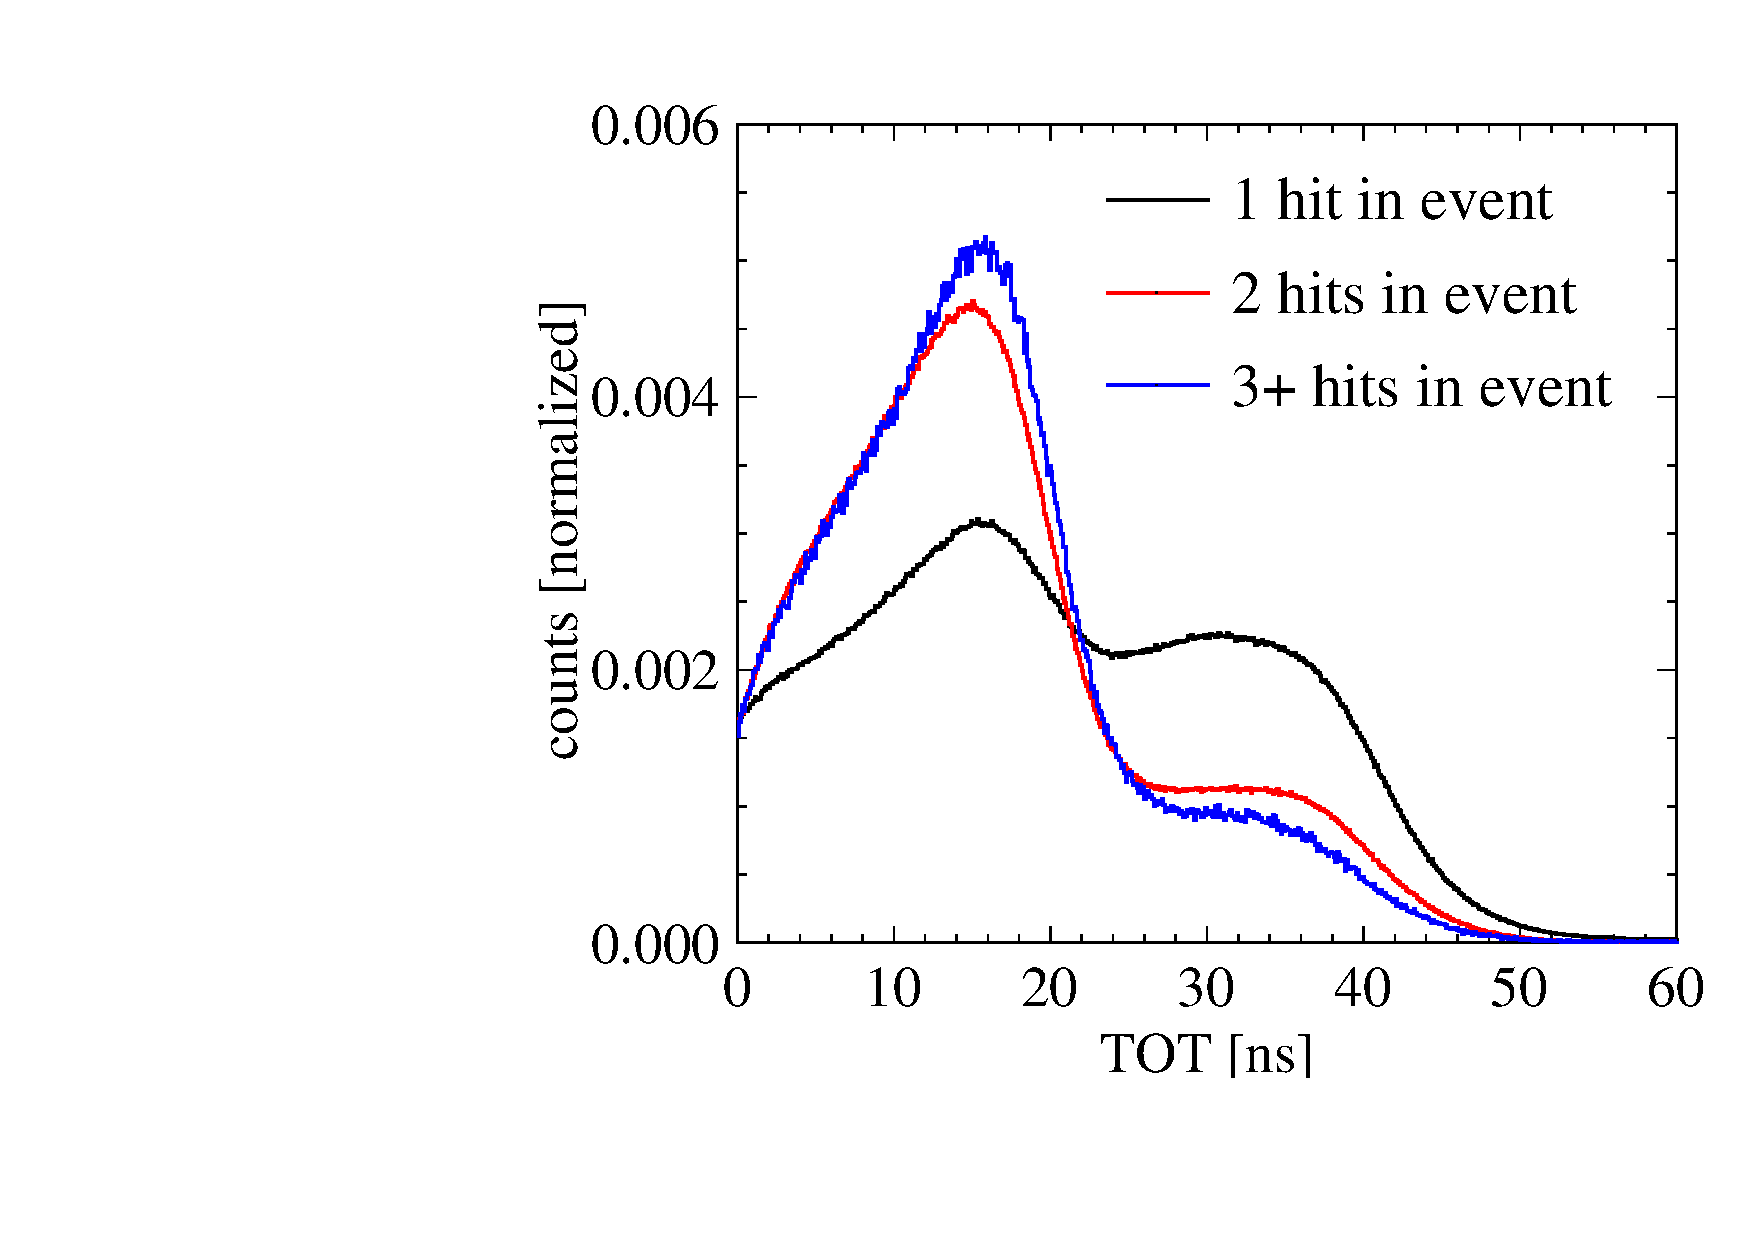
\includegraphics[width=0.45\textwidth]{Chapter8_analysis_jpet/img/tots_normalized}};
    \draw[black, thick, dashed] (1.25, 0.8) -- (1.25,5);
    \draw[black, thick, dashed] (2.98, 0.8) -- (2.98,5);
    \draw[black!60!white, ultra thick, <->] (1.25, 1.3) -- (2.98, 1.3);
  \end{tikzpicture}
  \caption{Distributions of time over threshold (TOT) values calculated for $\gamma$ interactions in all J-PET detection modules, before (left) and after calibration (right). Different colors denote TOT values of $\gamma$ hits observed in groups of 1, 2 and more within a 2.5~ns event time window. In the right panel the region of TOT used to select annihilation photon candidates is marked with dashed lines and a gray arrow.}\label{fig:tot_calib}
\end{figure}

\fref{fig:tot_calib} shows a comparison of the total TOT spectra from the whole detector before and after calibration. The distributions are presented separately for three classes of events, where an event is a set of hits contained within a narrow time window of 2.5~ns. In~cases where only one $\gamma$ interaction was recorded in a time window, the probability that the observed hit corresponds to~a high-energy deexcitation photon (1275~keV for the $^{22}$Na isotope used in the measurement) is almost even with the chance of observing a photon from annihilation. Conversely, for an increasing number of hits required in coincidence, the influence of high-energy photons on the TOT spectrum is decreased. Although slopes corresponding to Compton edges are visible in the TOT distributions both before and after calibration, its application results in a better separation of the structures from Compton spectra for photons from annihilation and deexcitation as well as in sharper Compton edges. This, in turn, allows for imposing requirements on the TOT value for identification of annihilation photon candidates as discussed in the next Section.

\subsection{3$\gamma$ event selection}\label{sec:3g_selection}
The preselection of data only required presence of at least three $\gamma$ interactions (hits) in a broad time window of 20~ns. Calibrated TOT values allow for restricting the further considerations to hits whose deposited energy, measured as TOT, could correspond to a~photon from 3$\gamma$ annihilation. Therefore, in further analysis only the hits whose TOT satisfied the following criterion:
\begin{equation*}
 0.5\ \text{ns} < TOT_{\gamma} < 20\ \text{ns},
\end{equation*}
(where the lower limit is introduced to reject poorly reconstructed hits) were considered as annihilation photon candidates. Similarly, location of the measured TOT$_{\gamma}$ value in the rightmost part of the TOT spectra presented in~\fref{fig:tot_calib} may be used to identify candidates for interactions of high-energy deexcitation quanta.
%
% TODO: dopisać, że prompty nie analizowane bo nie mają znaczenia bez o-Ps
%

In order to accommodate all possible $3\gamma$ event topologies and account for time resolution effects without allowing an excess of accidental coincidences, a time window width of 2.5~ns was chosen for further studies. A set of hits contained within such a time window will be later on referred to as an \textit{event}. Multiplicity of identified annihilation photon candidates observed in a single event is presented in~\fref{fig:hit_multiplicity}. Although further selection of hits corresponding to a single $3\gamma$ annihilation
is possible
in case 4 and more interactions were recorded in~coincidence,
the analysis presented in this work was restricted to events with exactly three annihilation photon candidates to avoid combinatorial issues.
\begin{figure}[h!]
  \centering
  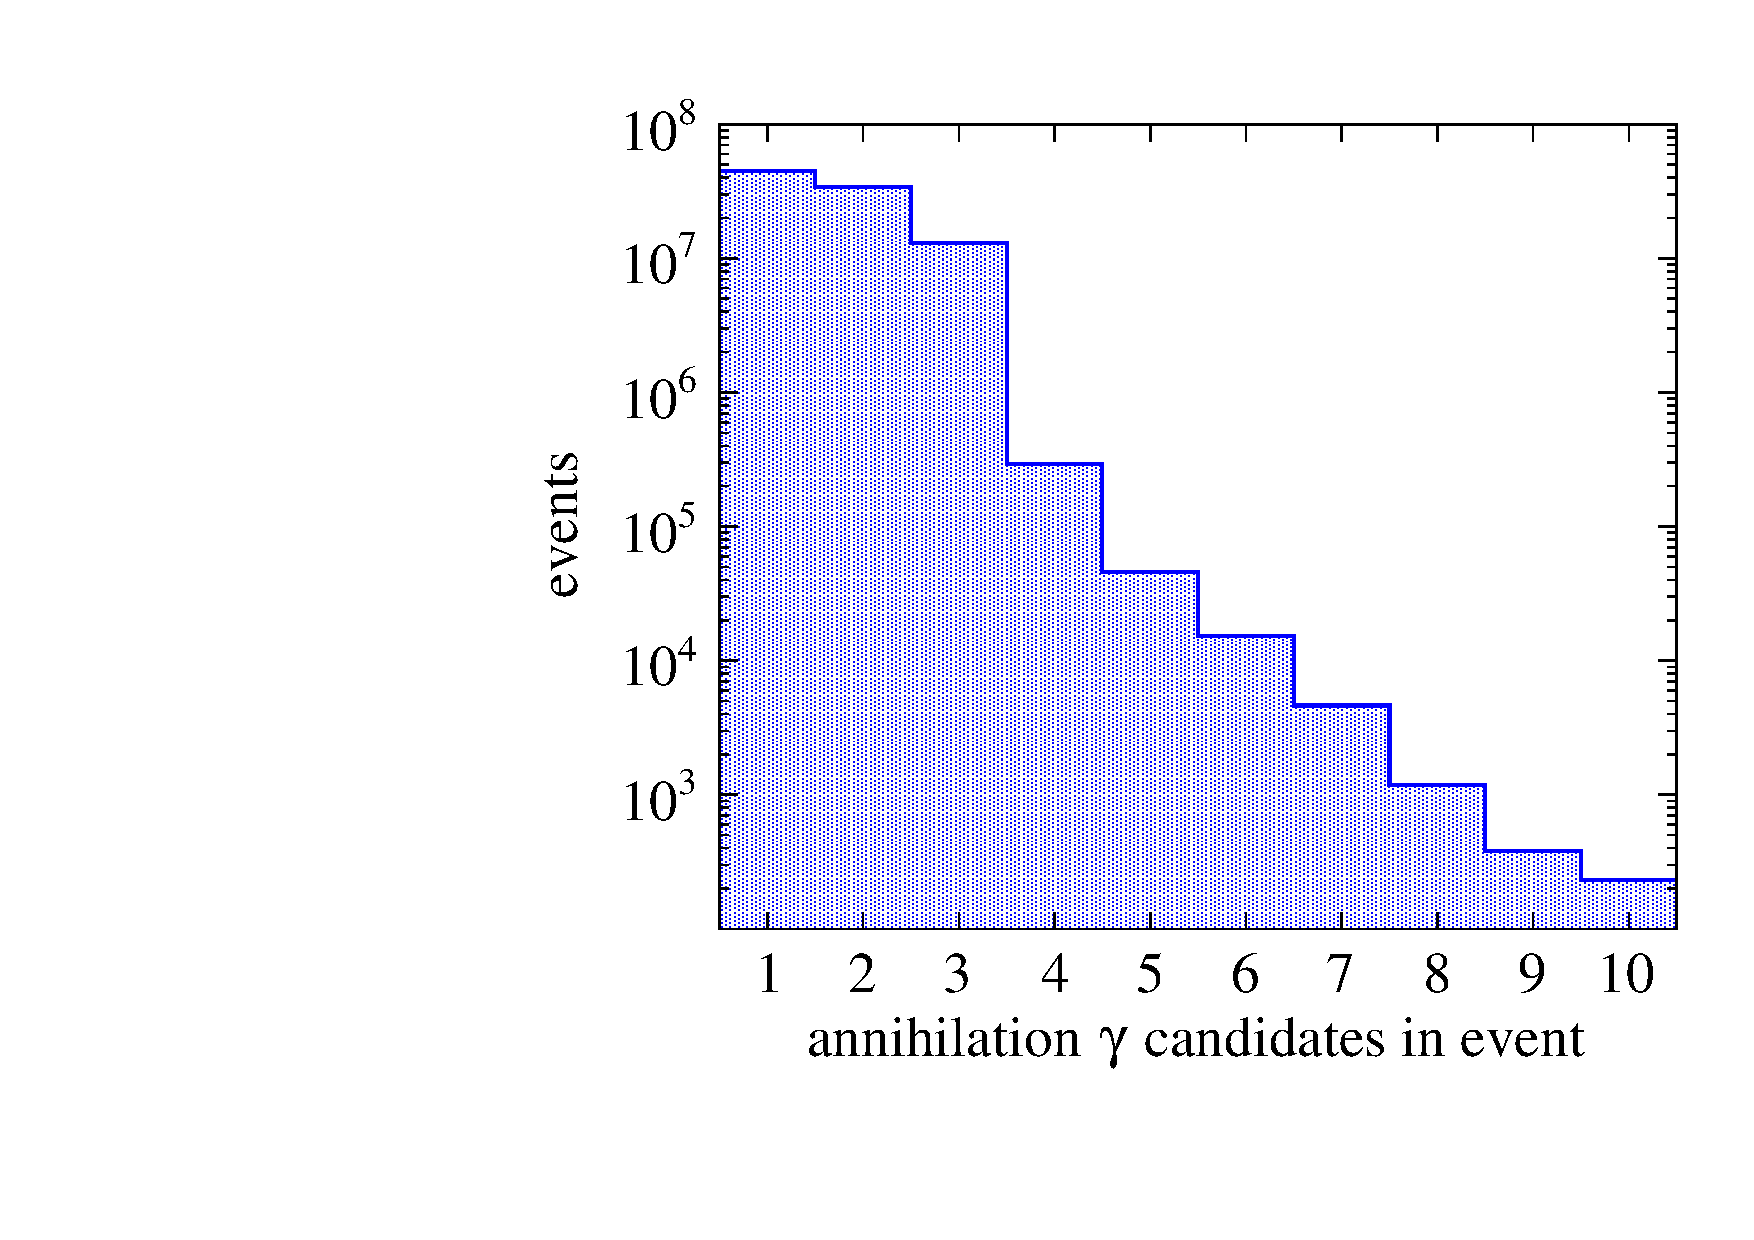
\includegraphics[width=0.45\textwidth]{Chapter8_analysis_jpet/img/anh_candidates}
  \caption{Multiplicity of annihilation photon candidates (identified using TOT) in a 2.5~ns time window.}\label{fig:hit_multiplicity}
\end{figure}

One of the major sources of background in the search for 3$\gamma$ annihilations in J-PET comes from secondary interactions of primary photons Compton-scattered in the scintillators. Registration of such scattered quanta is most probable in the detection modules directly neighboring the ones where the primary photon interacted, therefore events were rejected if they contained a pair of modules whose azimuthal coordinates were closer than \SI{8}{\degree}. Such criterion removes possible scatterings in modules next to each other in a single detector layer as well in pairs neighboring between the layers.

The second selection criterion targeting scattered photons was based on testing a hypothesis that the time difference between recorded hits corresponds to a time of flight of a photon between the two reconstructed $\gamma$ interaction positions. For all possible choices of 2 out of 3 hits in an event, the following variable was calculated:
\begin{equation}
  \label{eq:dvt}
  \delta t_{ij} = \abs{t_i - t_j} - \frac{1}{c}\abs{\vec{r}_i-\vec{r}_j},
\end{equation}
where $t_i$ and $\vec{r}_i$ denote respectively the recording time and position vector  of $i$-th photon interaction in an event and $c$ is the velocity of light.
A value of $\delta t_{ij}$ close to zero corresponds to a pair of hits created by subsequent Compton scatterings of the same photon in different detection modules.
Distribution of $\delta t_{min}$, defined as the smallest (in terms of absolute value) of three possible $\delta t_{12}$, $\delta t_{13}$ and $\delta t_{23}$ values for each event is displayed in~\fref{fig:dvt}.
In order to avoid possible contamination of the 3$\gamma$ event sample with secondary scatterings, a three-hit event was rejected if its $\delta t_{min}$ was greater than 1.8~ns.

\begin{figure}[h!]
  \centering
  \begin{tikzpicture}
    \node[anchor=south west,inner sep=0] at (0,0) 
    {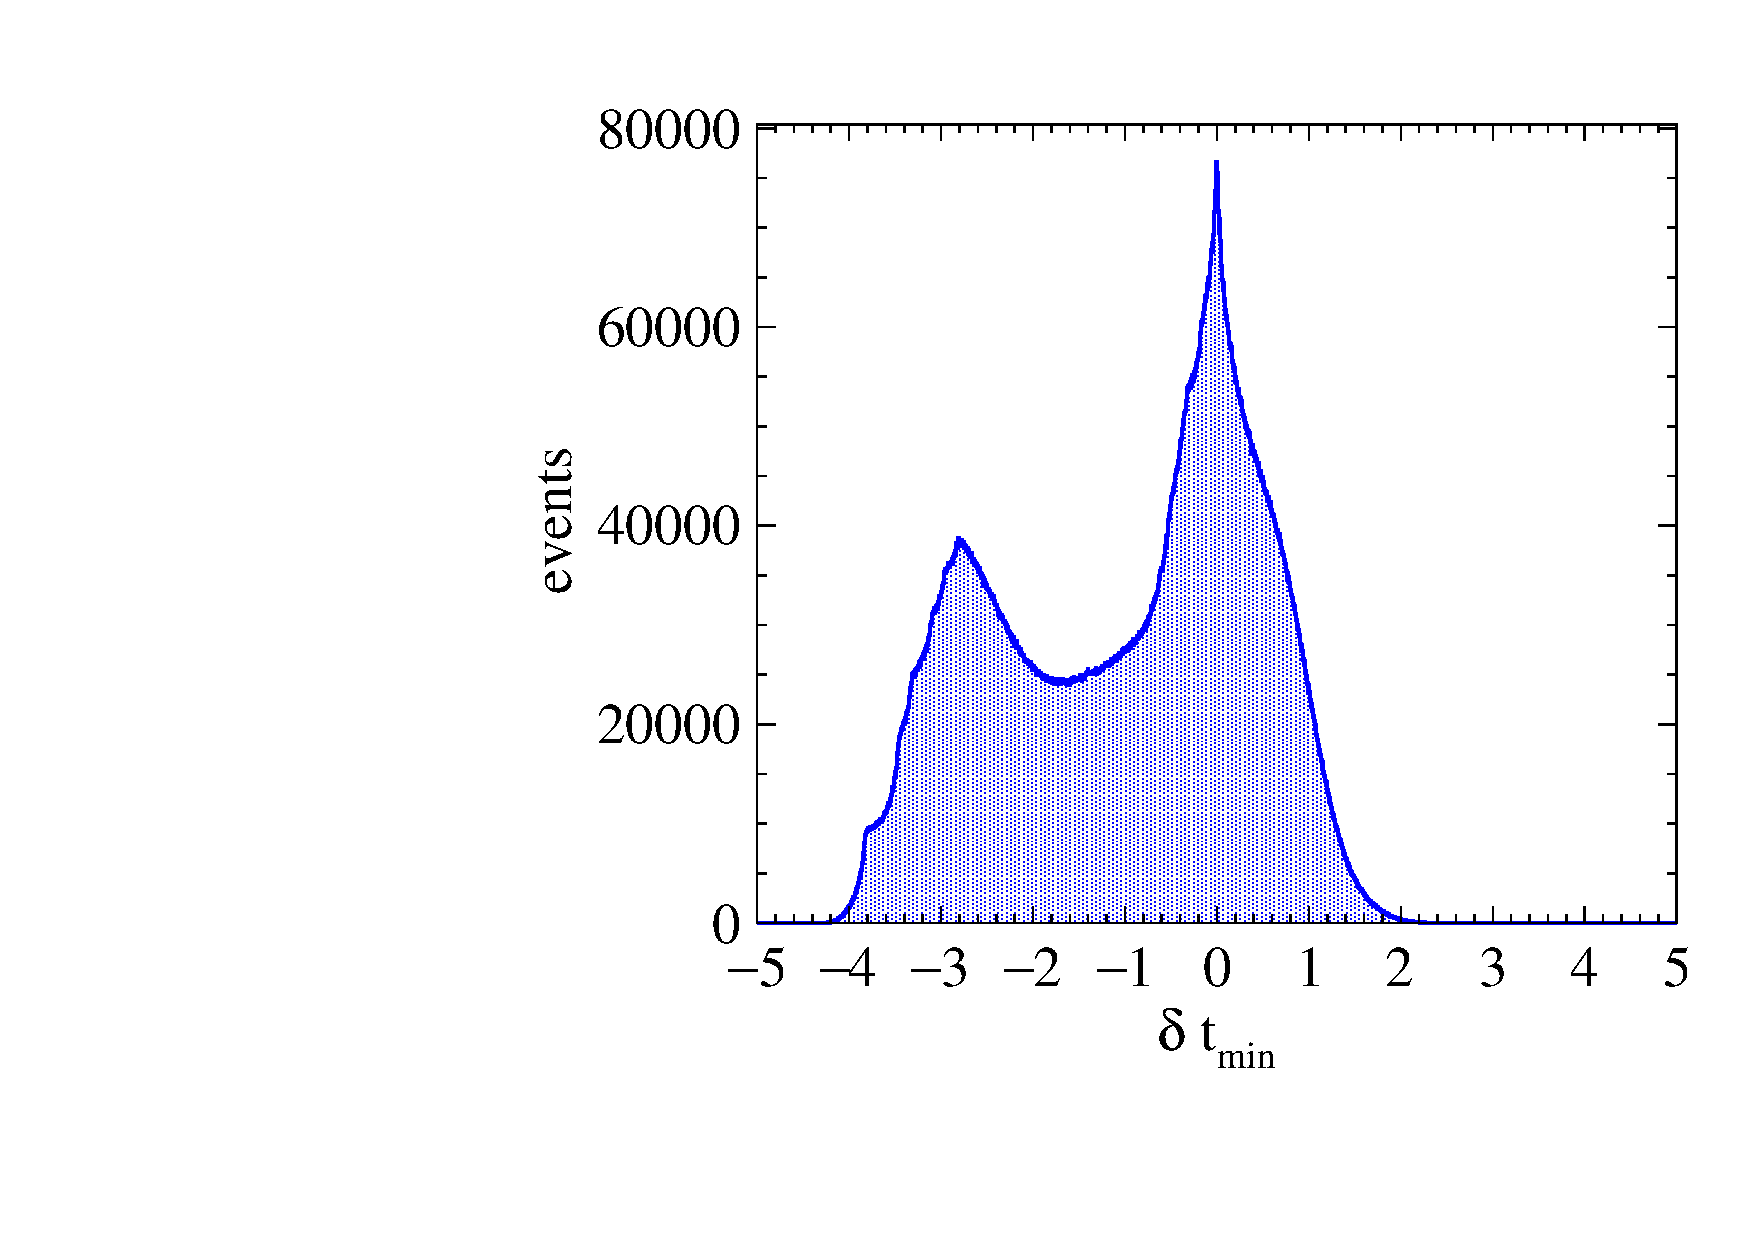
\includegraphics[width=0.45\textwidth]{Chapter8_analysis_jpet/img/delta_t_min}};
    \draw[black, thick, dashed] (3.0,0.9) -- (3.0,5.3);
    \node[] at (4.7, 0.25)  {[ns]};
    \draw[ultra thick, black!50!white, <->] (1.3, 3.5) -- (3.0, 3.5);
  \end{tikzpicture}    
  \caption{Distribution of the discrepancy between hits' recording times and their spatial separation divided by velocity of light, for the 2 out of 3 hits in an event which give a value closest to zero. Events with $\delta_{min} < 1.8$~ns are considered in further analysis as marked with the dashed line and gray arrow.}
  \label{fig:dvt}
\end{figure}

The last criterion imposed on the three-hit events to identify annihilations into three photons was based on the angular topology of the event. Preliminary studies with Monte-Carlo simulations had proven that 3$\gamma$ events can be distinguished from accidental coincidences of a 2$\gamma$ events with a third photon by the relative angles between the three photons' momenta~\cite{kowalski_scatter_fraction}.
Since the origin of the photons was not yet reconstructed at that stage, differences between azimuthal angles of the particular detection modules were used to calculate estimates of such relative angles, defined as:
\begin{equation}
  \label{eq:jpet_delta_theta}
  \delta \theta_{ij} = \abs{\theta_i - \theta_j}, \qquad ij=12,23,31,
\end{equation}
where $\theta_i$ is the azimuthal angle of the location of a detection module where $i$-th hit in an event was recorded. If such values of the three relative angles are labeled according to their descending order so that $\delta \theta_1 > \delta \theta_2 > \delta \theta_3$, the two smallest angles constitute useful variables in the 3$\gamma$ and 2$\gamma$ event discrimination. \fref{fig:jpet_angles} presents the relative distribution of the difference and sum of the two smallest relative $\theta$ angles. With such a choice of variables on the axes, events from two-photon annihilations, which contain two $\gamma$ quanta with opposite momenta, are clustered in a vertical band around $\delta\theta_2 + \delta \theta_3 \approx 180^{\circ}$. The 3$\gamma$ annihilations, on the other hand, are characterized by a large value of the sum of smallest angles and thus only events with:
\begin{equation*}
  \delta \theta_2 + \delta \theta_3 > 205^{\circ},
\end{equation*}
were considered as 3$\gamma$ candidates and subjected to the trilaterative reconstruction of the annihilation point as described in~\sref{sec:jpet_3g_imaging}. However, before the reconstruction results are presented, effects of imaging with two-photon annihilations using the same measurement will be briefly discussed as a useful benchmark for the study of 3$\gamma$ events.

\begin{figure}[h!]
  \centering
  \begin{tikzpicture}
    \node[anchor=south west,inner sep=0] at (0,0) 
    {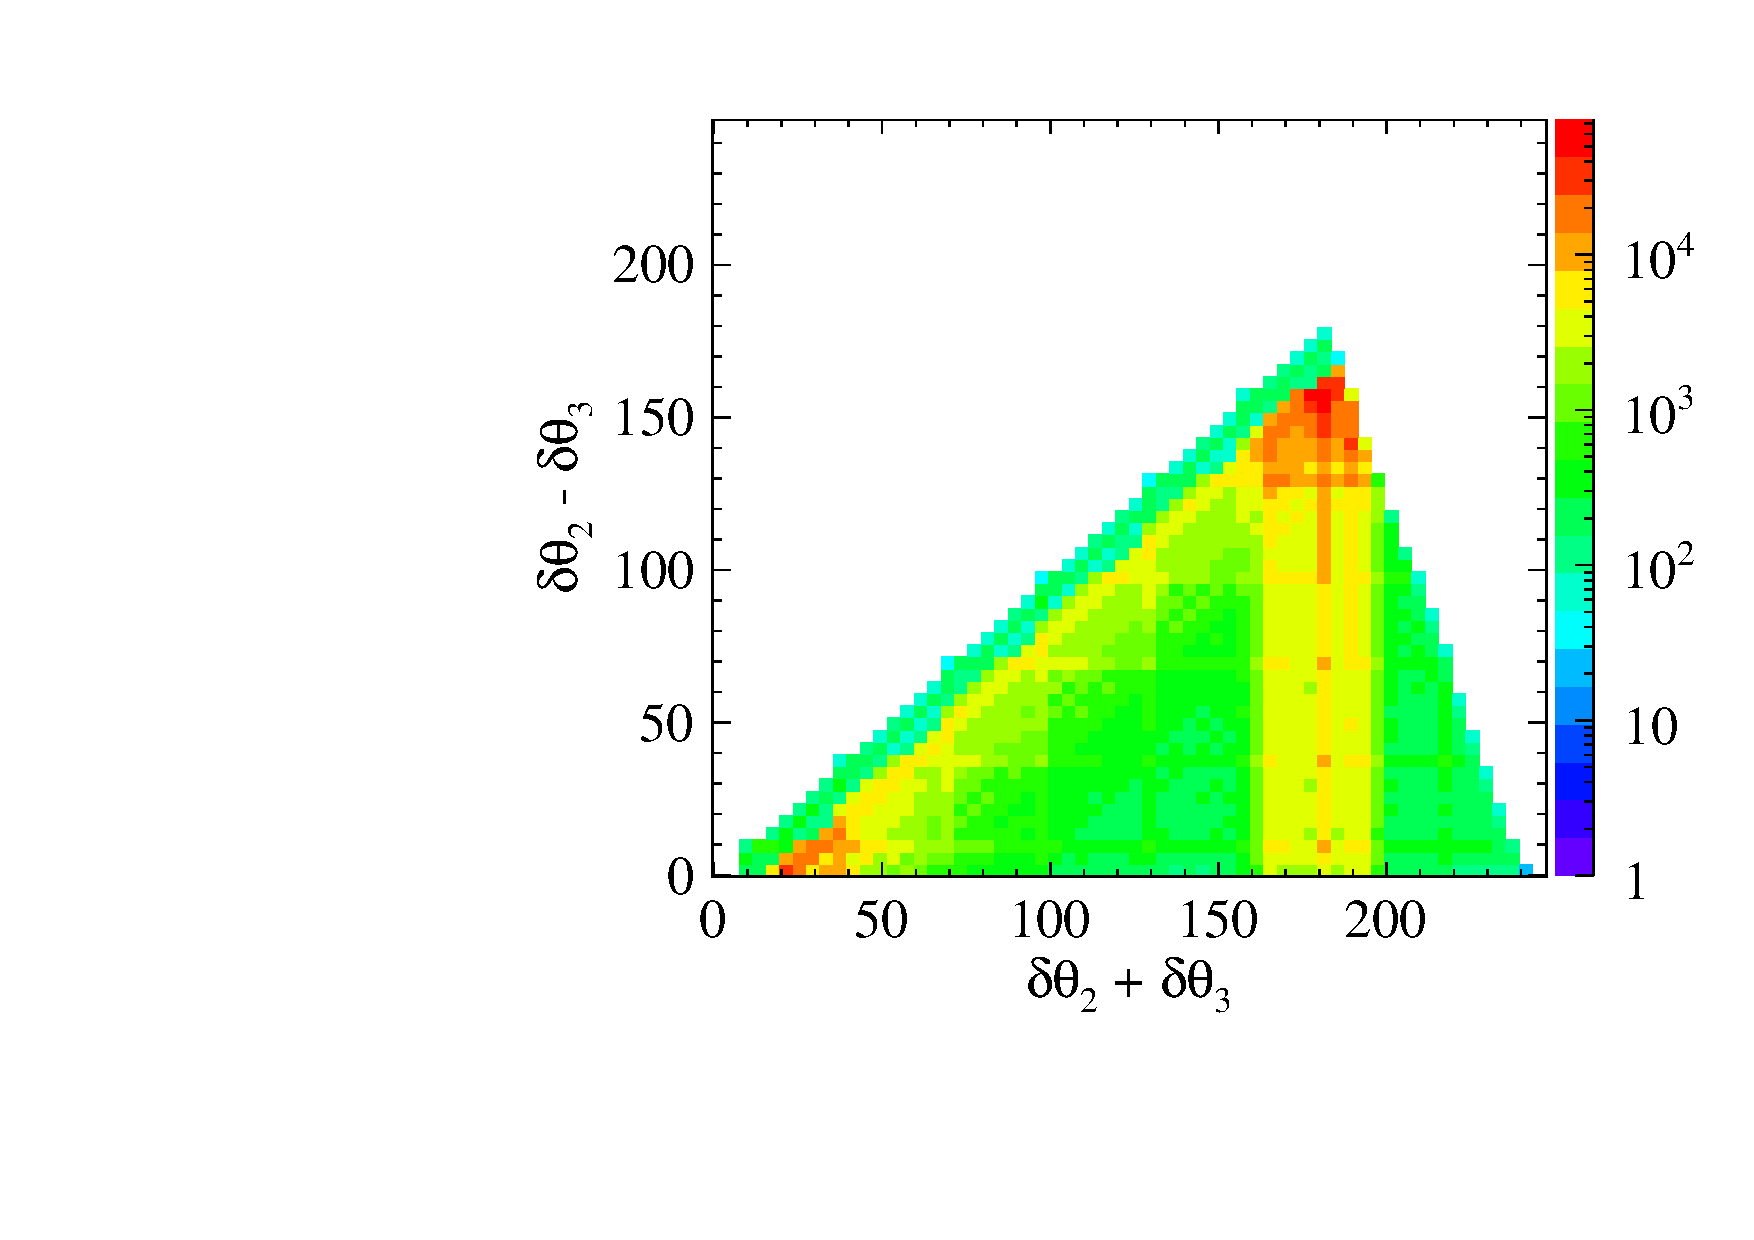
\includegraphics[width=0.45\textwidth]{Chapter8_analysis_jpet/img/angles}};
    \draw[black, thick, dashed] (5.0,0.9) -- (5.0,5.3);
    \draw[ultra thick, black!50!white, <->] (5.0, 3.5) -- (5.8, 3.5);
  \end{tikzpicture}  
  \caption{Relative distribution of the sum and difference of the two smaller azimuthal angles between three detection modules where hits were recorded in an event ($\delta\theta_1 > \delta\theta_2 > \delta\theta_3$). Events located to the right of the dashed line are selected as 3$\gamma$ annihilation candidates.}\label{fig:jpet_angles}
\end{figure}

\subsection{Benchmark imaging of the 3$\gamma$ production chamber with 2$\gamma$ annihilations}
\label{sec:2g_imaging}
In order to understand the limits of available reconstruction of points of annihilation taking place in the wall of the 3$\gamma$ production chamber, classical tomography with $e^+e^-$ annihilations to two photons may be used as a benchmark. Due to the probability of such annihilations larger by over two orders of magnitude than in case of direct annihilation to 3$\gamma$ as well as simple back-to-back configuration of the photons' momenta, a pure sample of such events is selected more easily at the same time yielding larger statistics for the reproduction of the chamber tomographic image.

About \SI{15}{\percent} of the data taken in the test run were analyzed using the procedures devised for tomographic imaging with J-PET. Identified two-photon annihilation events were used to reconstruct lines of response
\footnote{In PET tomography, a line of response is a line connecting two places of photon interactions recorded in the detector, on which the 2$\gamma$ annihilation point must be located.}
(LORs) and difference between each photon time of flight allowed to find the annihilation point along a LOR. Detailed description of the applied imaging procedure may be found in Reference~\cite{monika_2gamma_imaging}. Thus obtained tomographic images of the aluminum chamber as well as the $\beta^+$ source setup used in the measurement are presented in~\fref{fig:2g_image}. This benchmark images lead to two observations useful for further analysis of for 3$\gamma$ reconstruction performance. Firstly, it is visible that the largest amount of $e^+e^-$ annihilations take place directly in elements of the setup supporting the $^{22}$Na source (see~\fref{fig:jpet-source}, right), located at $z=0$. Therefore, a clear observation of the reconstruction of annihilations originating in the chamber walls requires exclusion of its central part where the source was mounted. \fref{fig:2g_image_c} shows the transverse plane location of $2\gamma$ annihilation points whose longitudinal coordinate satisfied:
\begin{equation*}
  \abs{z} > 4\ \text{cm},
\end{equation*}
in which case annihilations taking place in the chamber material are clearly visible.
A similar requirement will be used for the demonstration of $3\gamma$ annihilations' reconstruction discussed in the next Section.

\begin{figure}[h!]
  \centering
%  \captionsetup[sub]{margin=1ex}
  \captionsetup[subfigure]{justification=centering}
  \begin{subfigure}{0.45\textwidth}
  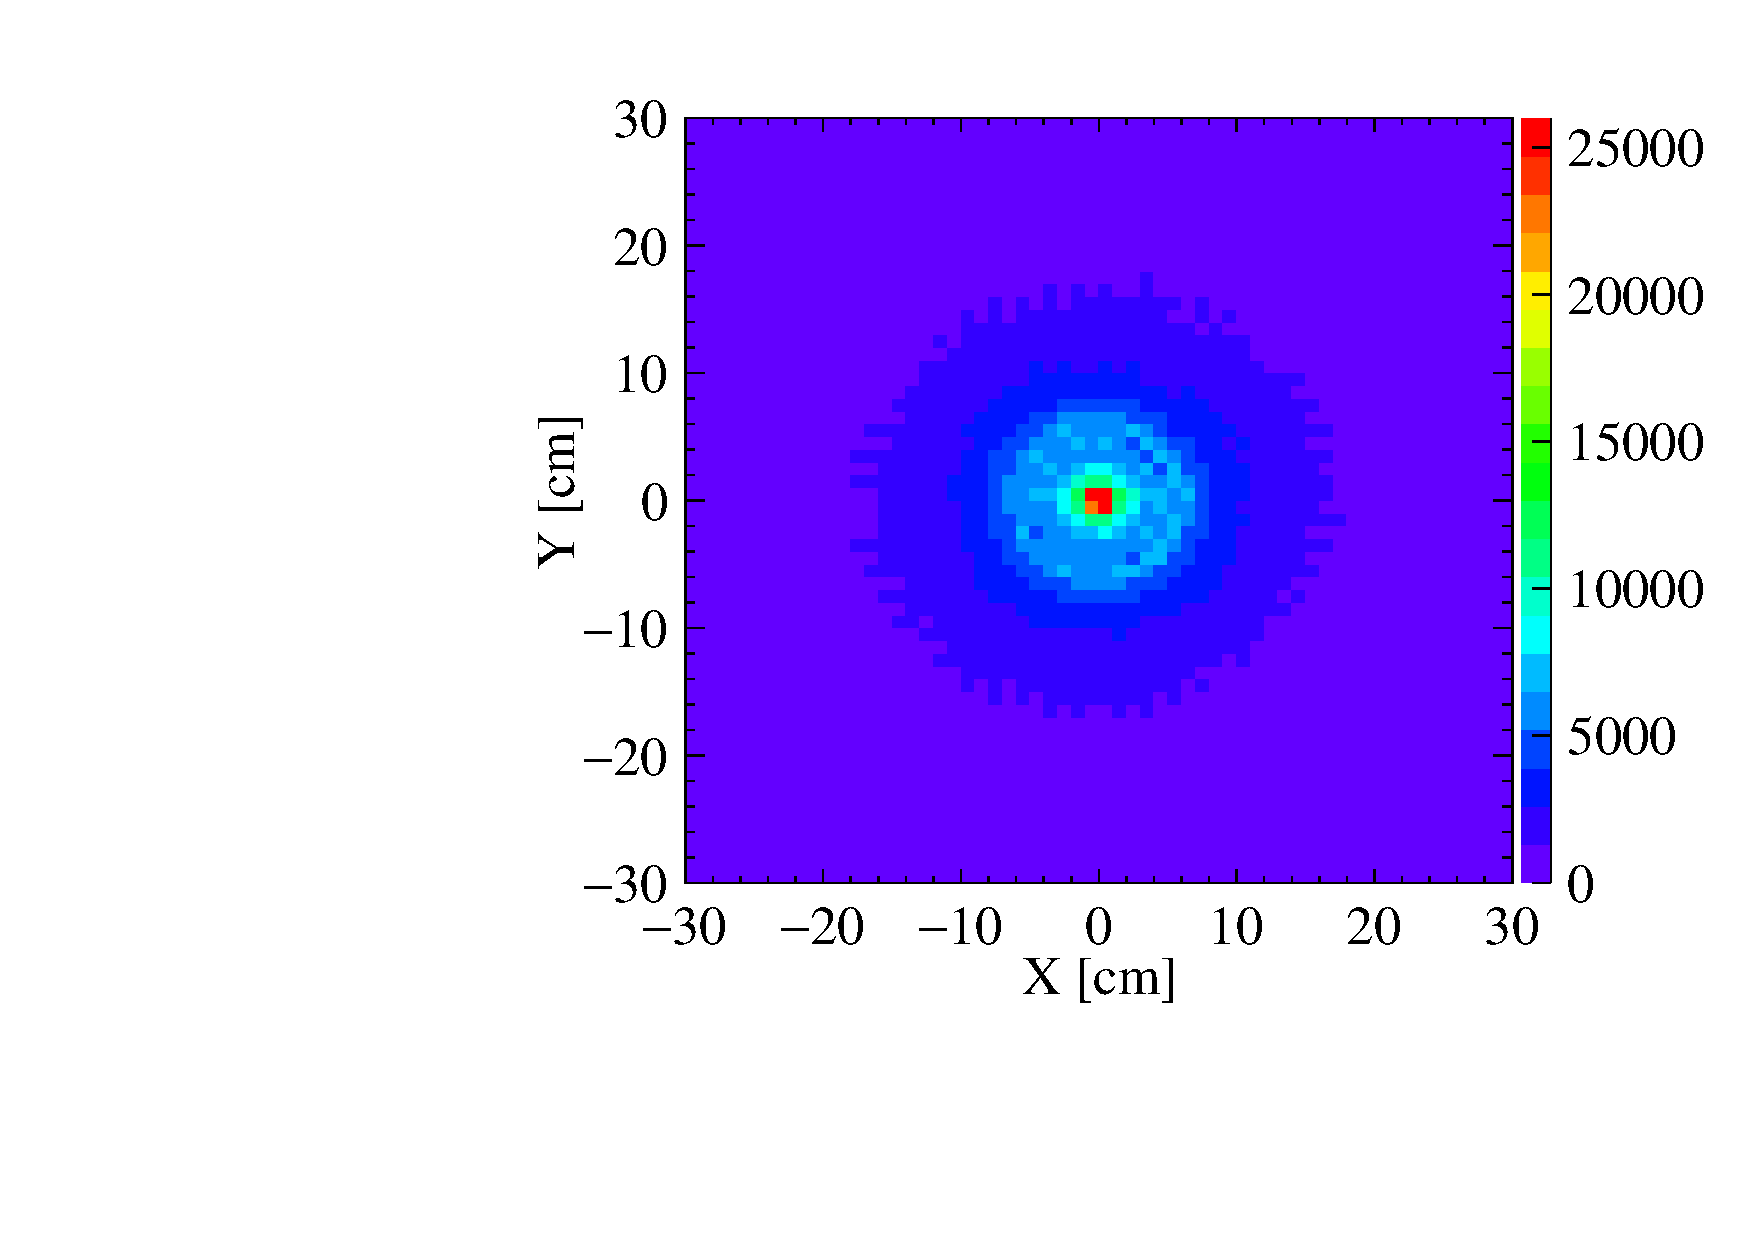
\includegraphics[width=1.0\textwidth]{Chapter8_analysis_jpet/img/2g_xy_all}
  \caption{Transverse view image,\\ all $z$ values projected}\label{fig:2g_image_a}
  \end{subfigure}
  \hspace{1em}
  \begin{subfigure}{0.45\textwidth}
  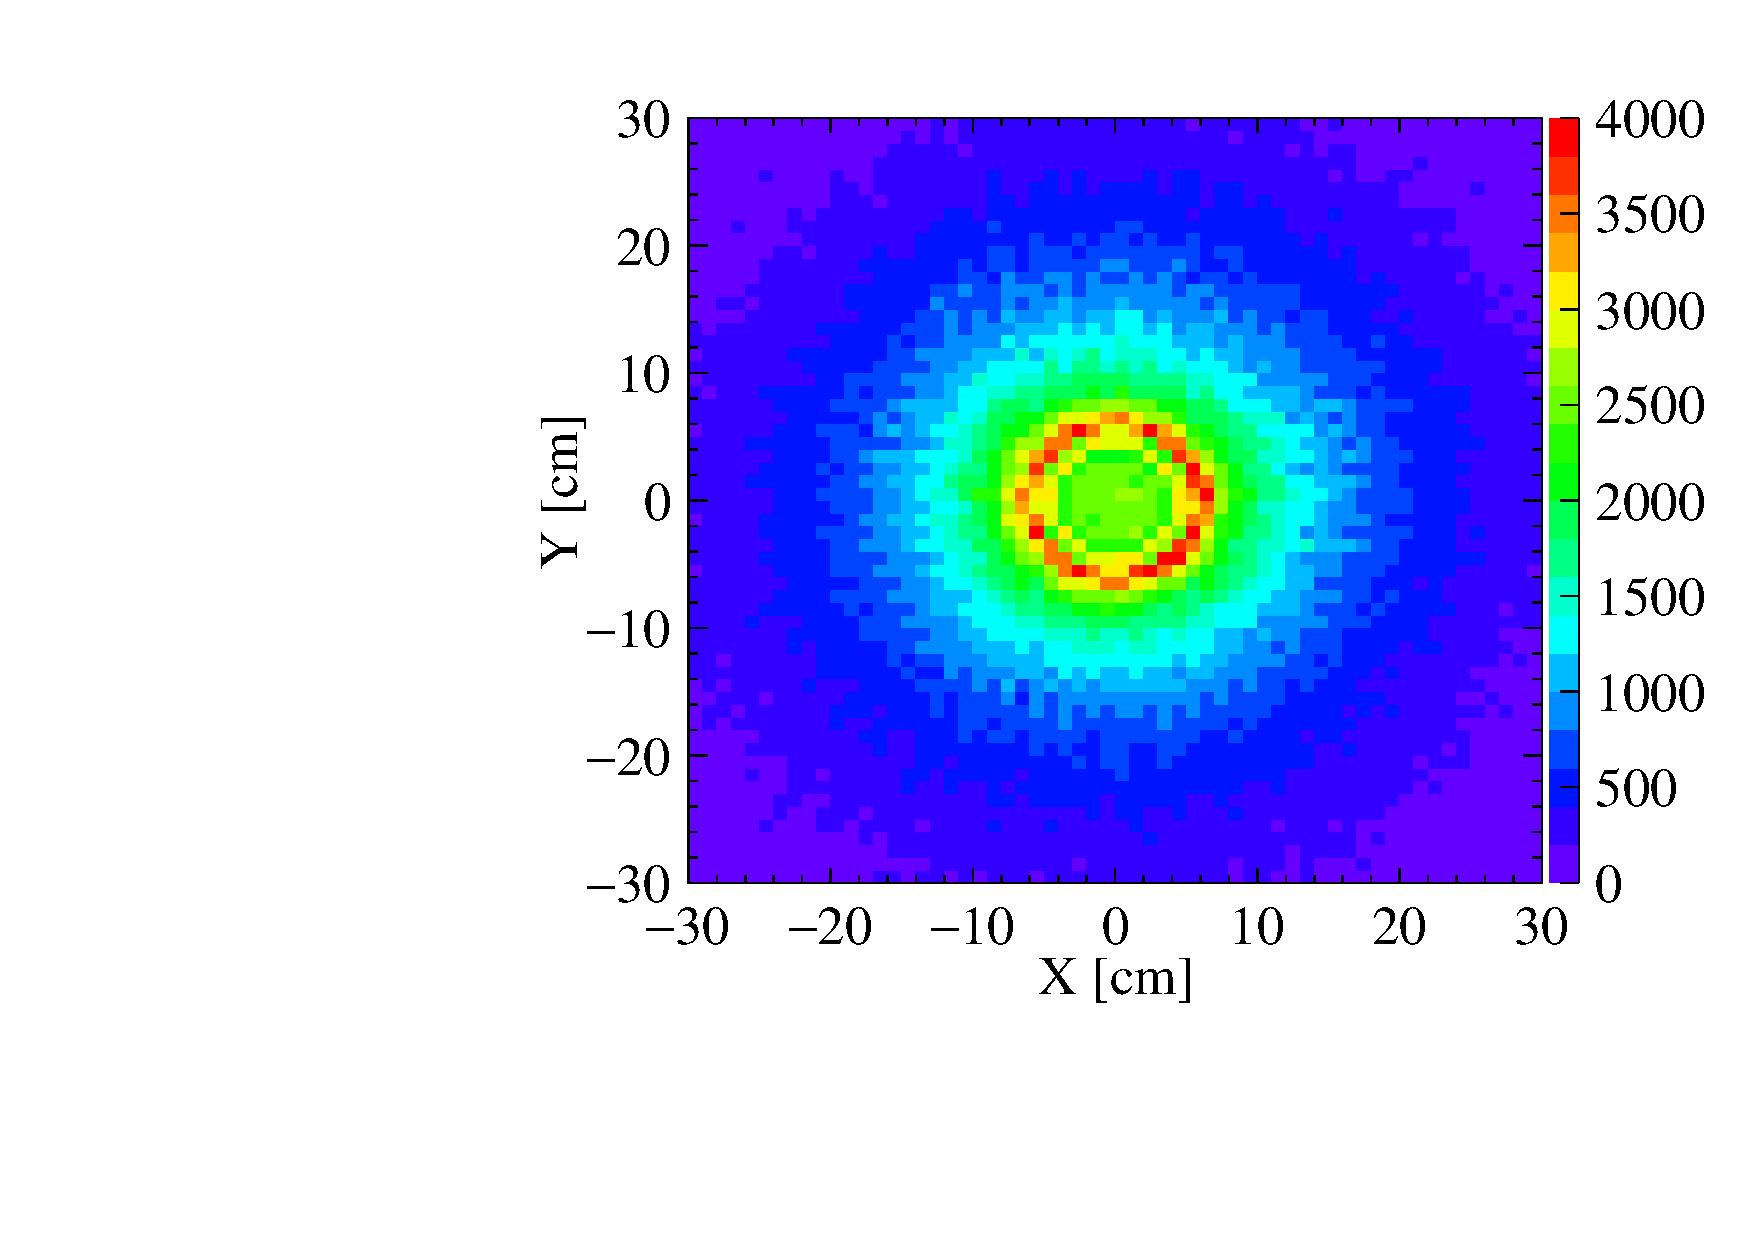
\includegraphics[width=1.0\textwidth]{Chapter8_analysis_jpet/img/2g_xy_nocenter}
  \caption{Transverse view image,\\ $\abs{z} > 4$~cm}\label{fig:2g_image_c}
\end{subfigure}
  \begin{subfigure}{0.45\textwidth}
  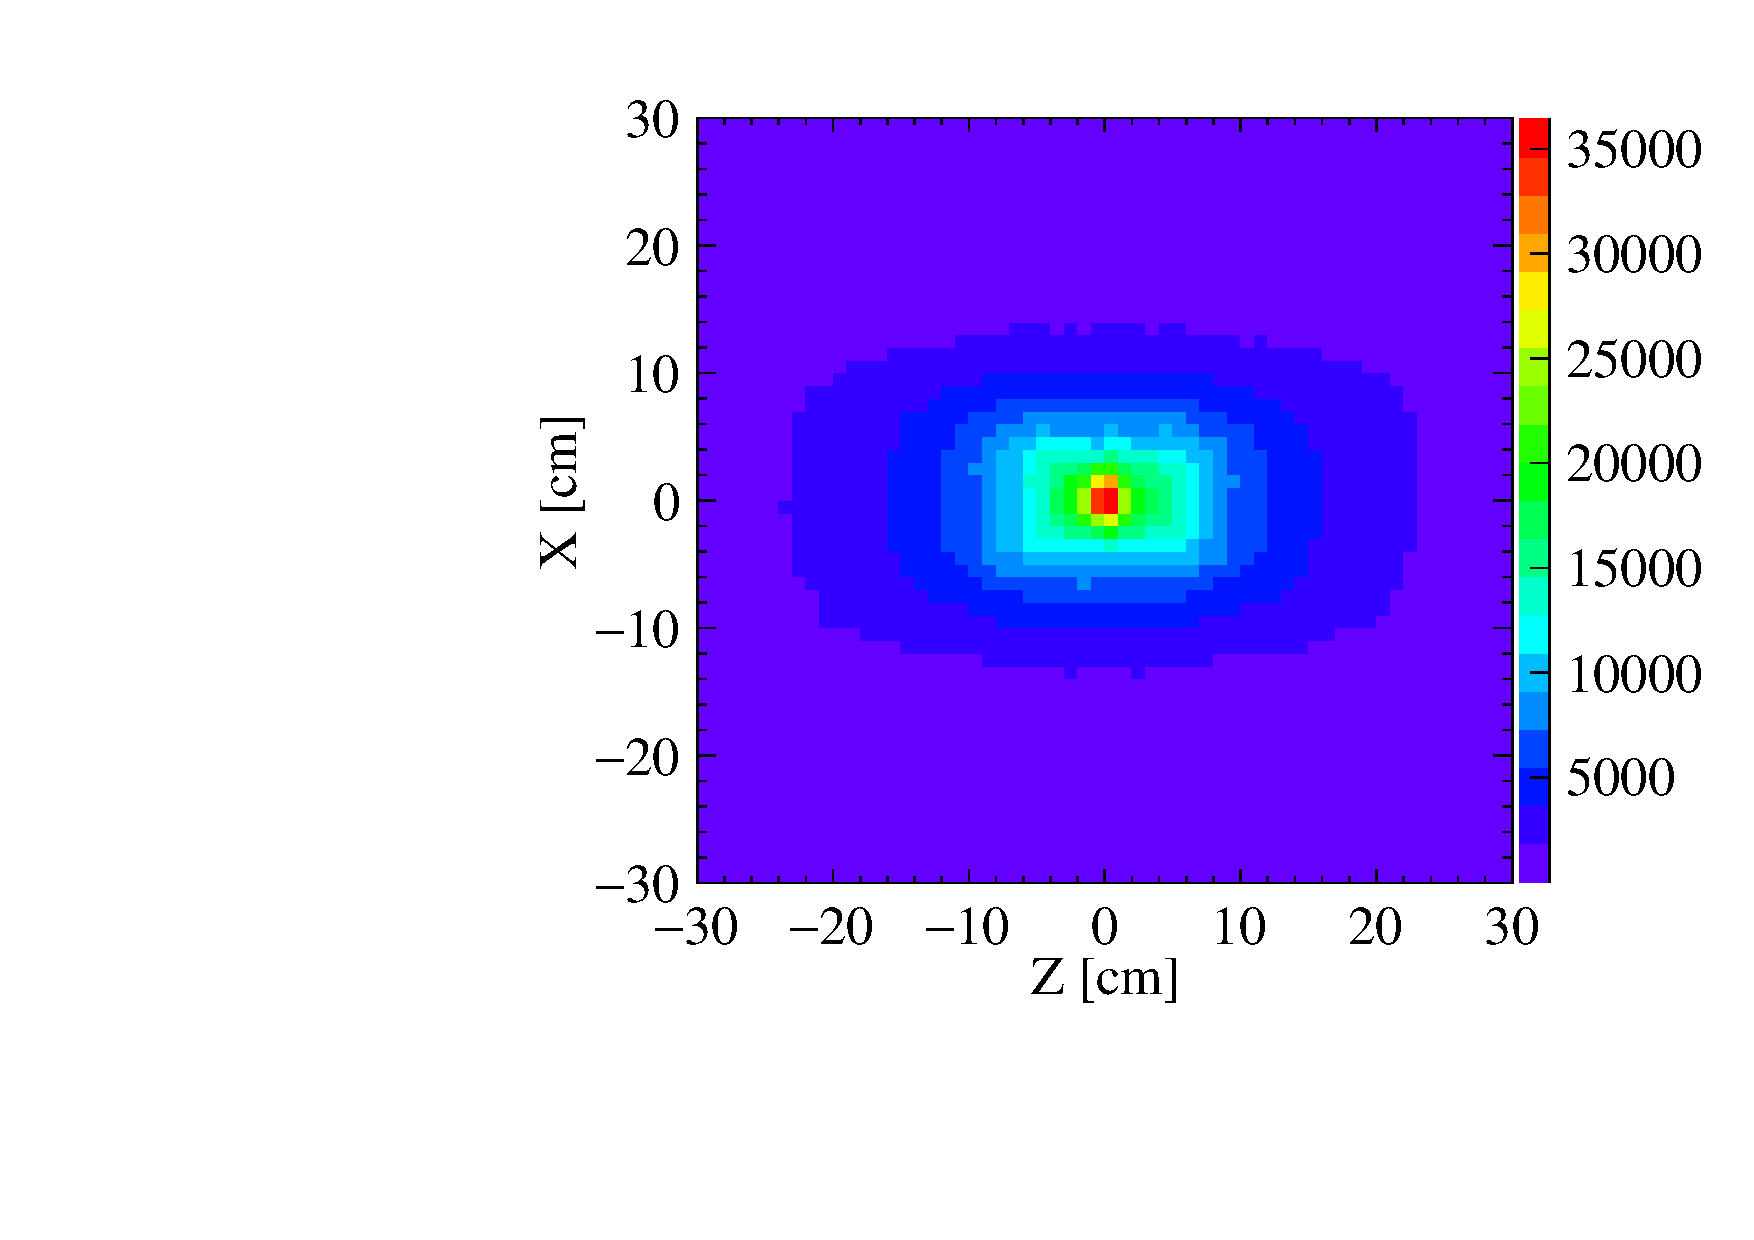
\includegraphics[width=1.0\textwidth]{Chapter8_analysis_jpet/img/2g_xz_all}
  \caption{Side view image}\label{fig:2g_image_b}
\end{subfigure}
  \caption{Tomographic images of the annihilation target cylinder and $\beta^+$ source obtained using $e^+e^-\to 2\gamma$ annihilations used as a benchmark for the 3$\gamma$ annihilation reconstruction studies.}\label{fig:2g_image}
\end{figure}

Second conclusion following from the benchmark $2\gamma$ images is the size of the effective sensitive volume inside the detector along the $z$ coordinate. Although the aluminum chamber spanned the whole length of the latter, \fref{fig:2g_image_b} reveals that only in the region of about~$|z| < 8$~cm the annihilations in the chamber material are efficiently reproduced. This is caused by two geometrical effects:
\begin{itemize}
\item for larger $z$ values, a constant element of the chamber wall surface corresponds to a smaller solid angle of positrons' emission from a point-like source; a decrease of $e^+e^-$ annihilation rate is thus expected with increasing distance from the source along $z$,
\item the geometrical acceptance of the detector barrel is reduced for annihilations taking place closer to its edges.
\end{itemize}
The first argument, concerning rate of positron interactions in a section of the chamber wall surface, is directly relevant also in case of the 3$\gamma$ annihilations. The second factor, in case of two photon annihilations, results from the fact that after registration of one $\gamma$ quantum, the other one with opposite momentum must also reach a detector module.
\fref{fig:stereo} schematically depicts this geometrical acceptance limitations for a simplified case of annihilations originating on the detector $z$ axis.
Effectively, only $\gamma\gamma$ pairs emitted in a volume limited by two cones coaxial with the detector with an opening angle $\vartheta = \text{arctan}\frac{R_1}{L/2-z}$ (where $L$ is the scintillator length and $R_1$ is the radius of the innermost scintillator layer) can be registered.
The stereo angle corresponding to this volume is given by:
\begin{equation}
  \label{eq:stereo_angle}
  \Omega(z) = 2\int_{0}^{2\pi}d\phi \int_{\vartheta(z)}^{\pi/2} \sin\theta d\theta = 4\pi \cos\vartheta(z) = 4\pi\frac{\frac{L}{2}-z}{\sqrt{R_1^2+\left(\frac{L}{2}-z\right)^2}}.
\end{equation}
The above relation approximately describes the $z$-dependent decrease in the detection efficiency for recording 2$\gamma$ annihilations. Such considerations can also be used to approximate the drop in efficiency for 3$\gamma$ events if a decay plane is considered instead of the line constituted by two photons' opposite momenta. A conclusion which follows from the above benchmark is therefore that good performance of the reconstruction of three photon annihilations should be expected in approximately the same range as in case of the 2$\gamma$ benchmark image, i.e.\ for about $\abs{z} < 8$~cm.

\begin{figure}[h!]
  \centering
\begin{tikzpicture}[
  scale=0.5,
  >={Stealth[inset=0pt,length=6pt,angle'=50,round]}
  ]
  % dummy rect
  \draw[white] (-5.5,-6) rectangle (9,6);

  % cones
  \draw[fill, gray!30!white] (-1,4.1) -- (5, 4.1) -- (2.0, 0.0);
  \draw[fill, gray!30!white] (-1,-4.1) -- (5, -4.1) -- (2.0, 0.0);

  % photons
  \draw[->,decorate,decoration={snake, amplitude=0.4mm}] (2.0, 0.0) -- (5.0, 4.1);
  \draw[->,decorate,decoration={snake, amplitude=0.4mm}] (2.0, 0.0) -- (-1.0, -4.1);
  
  % detector
  \draw[<->] (-5,4.6) -- (5,4.6) node[midway, above] {\large L};
  \draw[fill=black!50!white] (-5,4.1) rectangle (5,4.3);% node[right] {\large Layer 1};

  \draw[fill=black!50!white] (-5,-4.3) rectangle (5,-4.1);
  
  \draw[line width=1pt,dotted, black, ->] (-5,0) -- (5.5,0) node[xshift=10] {\large Z};
  \draw[black, <->] (0,0.35) -- (2.0,0.35) node[midway, above] {\large $z$};
  \draw[line width=1pt] (0.0, -0.3) -- (0.0, 0.3) node[below, yshift=-7] {\large 0};

  % annihilation
  \draw[fill, black] (2.0, 0.0) circle (0.1);
  \node[] at (3.1,-0.6) {\large $\vartheta$};
  \draw[] (4.0, 0.0) arc(0:-53:2.0);
  
  % radius
  \draw[<->] (2.0, 0.0) -- (2.0, -4.1) node[midway, left, yshift=-5] {\large $R_1$};

  %
  \draw[<->] (2.0, -4.6) -- (5.0, -4.6) node[midway, below, yshift=0] {\large $\frac{L}{2} - z$};
  
\end{tikzpicture}
\caption{Schematic presentation of the geometrical acceptance limits on reconstruction of 2$\gamma$ annihilations along the $z$ axis of the detector. Shaded region denotes the volume in which emitted $e^+e^-$ pairs may be detected.}\label{fig:stereo}
\end{figure}

\subsection{Reconstruction of 3$\gamma$ annihilation points}
\label{sec:jpet_3g_imaging}
The selection of 3$\gamma$ events described in~\sref{sec:3g_selection} applied to the test measurement data yielded 1164 event candidates. For each candidate, the annihilation point was reconstructed using the trilateration-based method presented in~\sref{sec:gps_jpet}. Distributions of the resulting annihilation points are presented in~\fref{fig:3g_image}.
The transverse view images are shown separately for the complete projection along detector $z$ axis as well as for the region of $\abs{z}>4$~cm, i.e.\ excluding the volume were most annihilations originate in the support of the $\beta^+$ source rather than in the chamber walls as demonstrated with the 2$\gamma$ images.
\begin{figure}[h!]
  \centering
%  \captionsetup[sub]{margin=1ex}
  \captionsetup[subfigure]{justification=centering}
  \begin{subfigure}{0.45\textwidth}
  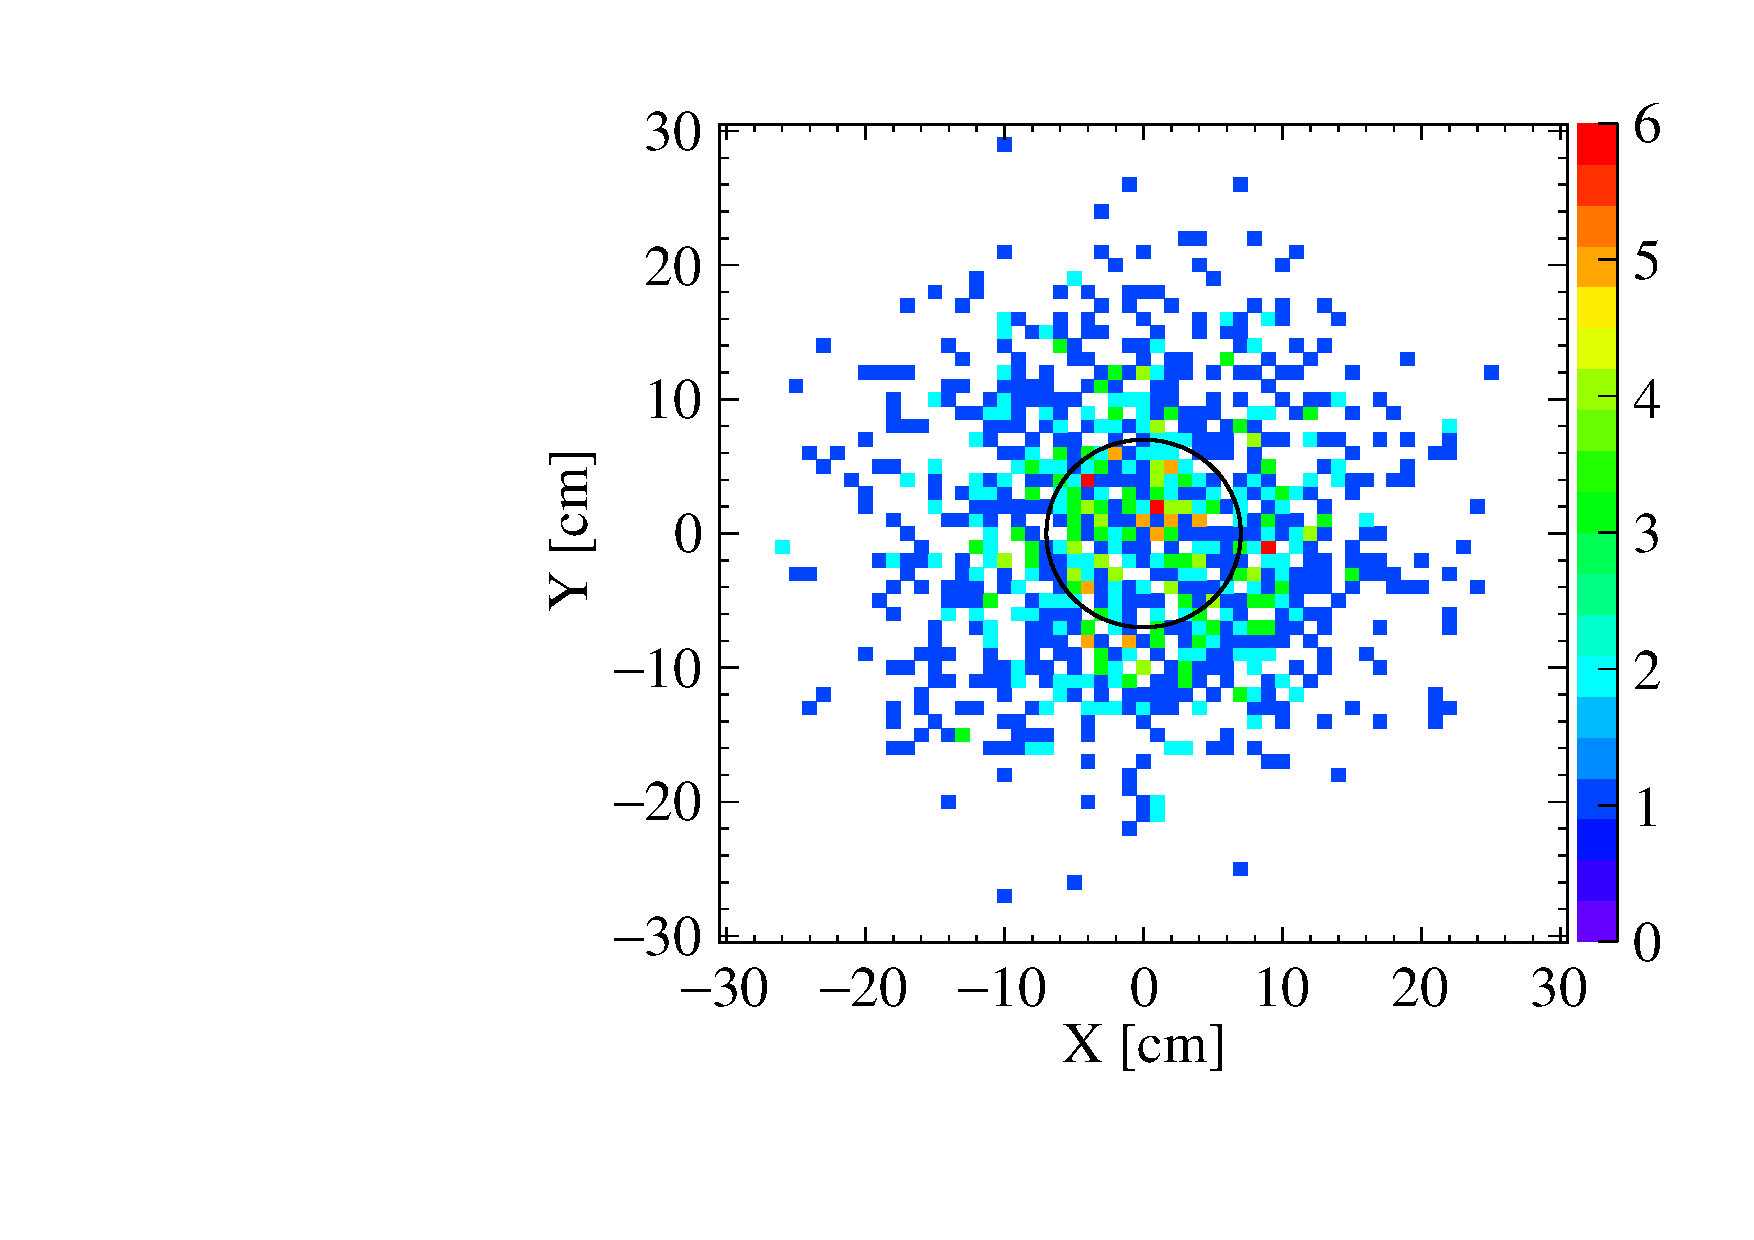
\includegraphics[width=1.0\textwidth]{Chapter8_analysis_jpet/img/3g_xy_all}
  \caption{Transverse view image,\\ all $z$ values projected}\label{fig:3g_image_a}
  \end{subfigure}
  \hspace{1em}
  \begin{subfigure}{0.45\textwidth}
  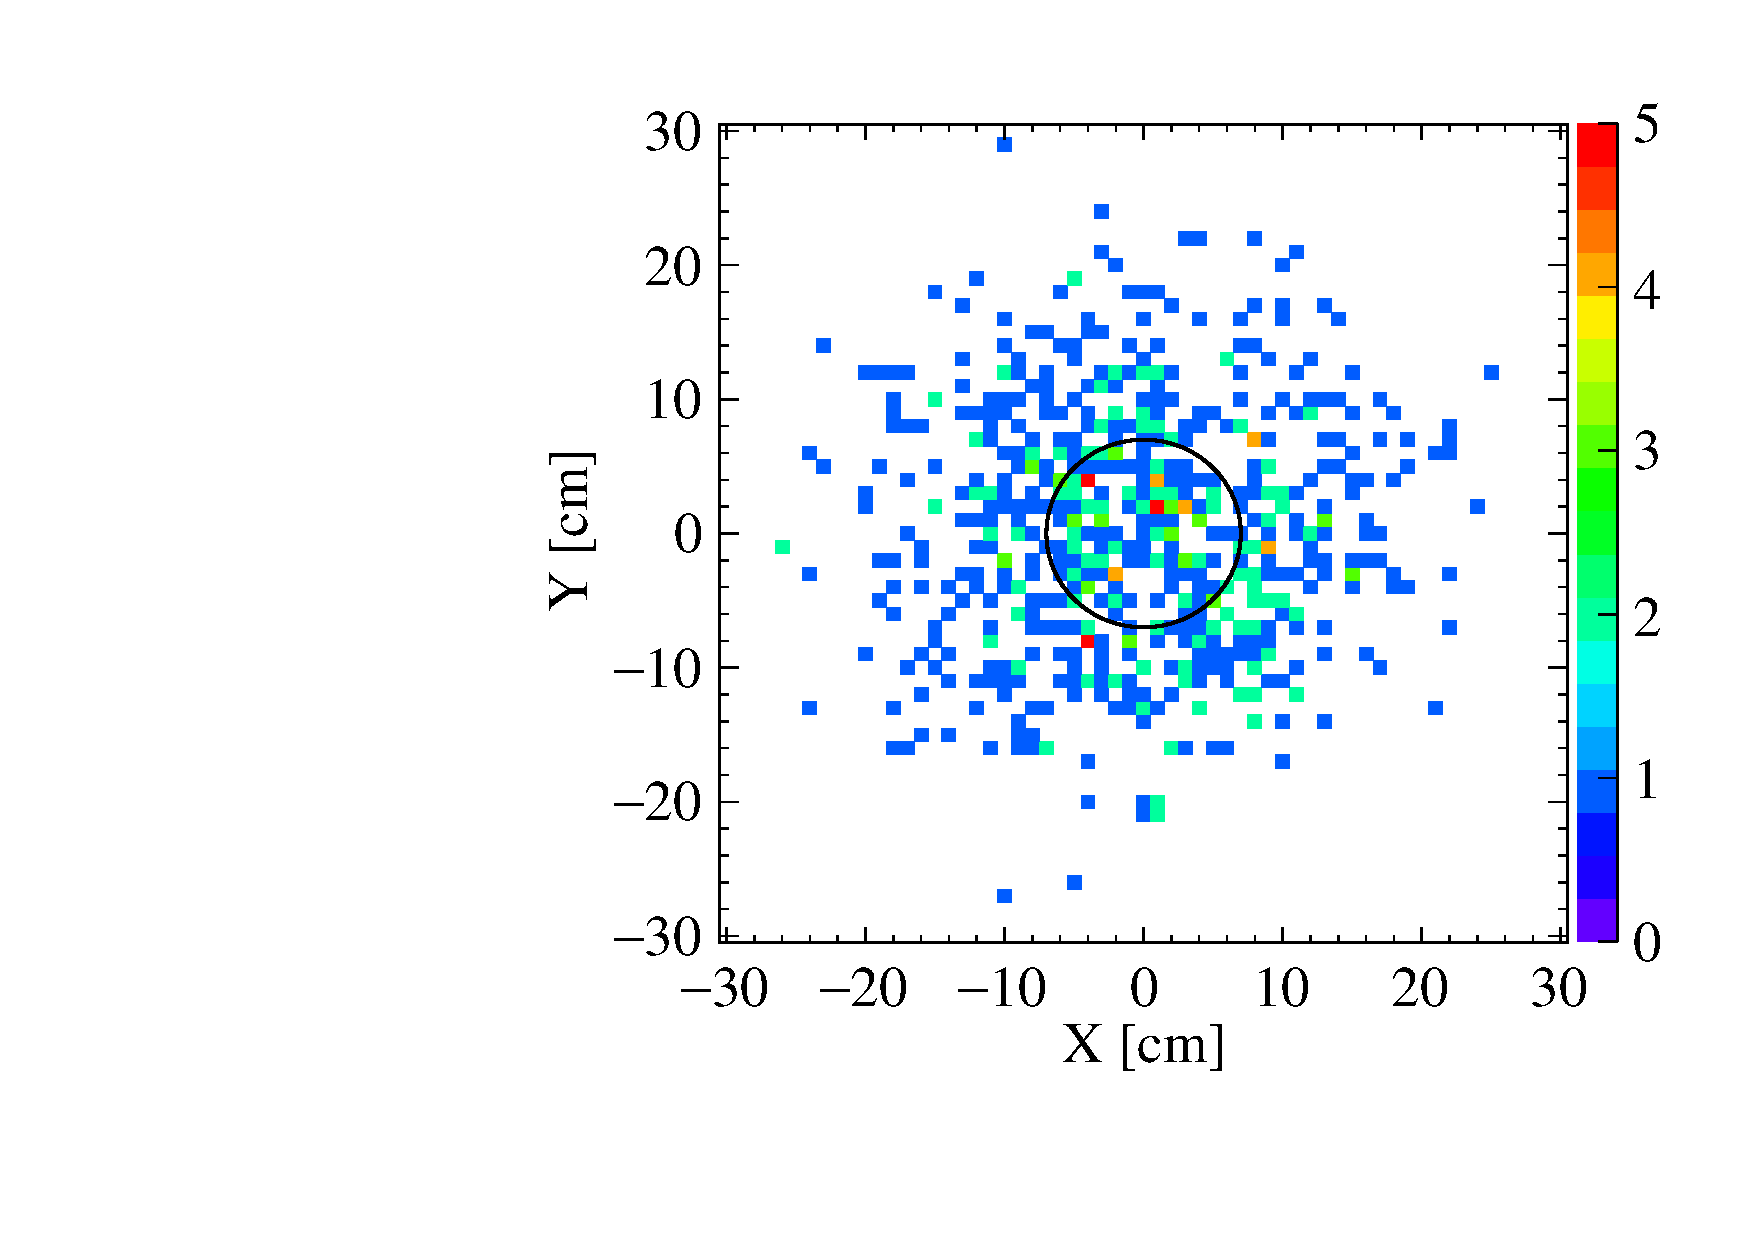
\includegraphics[width=1.0\textwidth]{Chapter8_analysis_jpet/img/3g_xy_nocenter}
  \caption{Transverse view image,\\ $\abs{z} > 4$~cm}\label{fig:3g_image_c}
\end{subfigure}
  \begin{subfigure}{0.45\textwidth}
  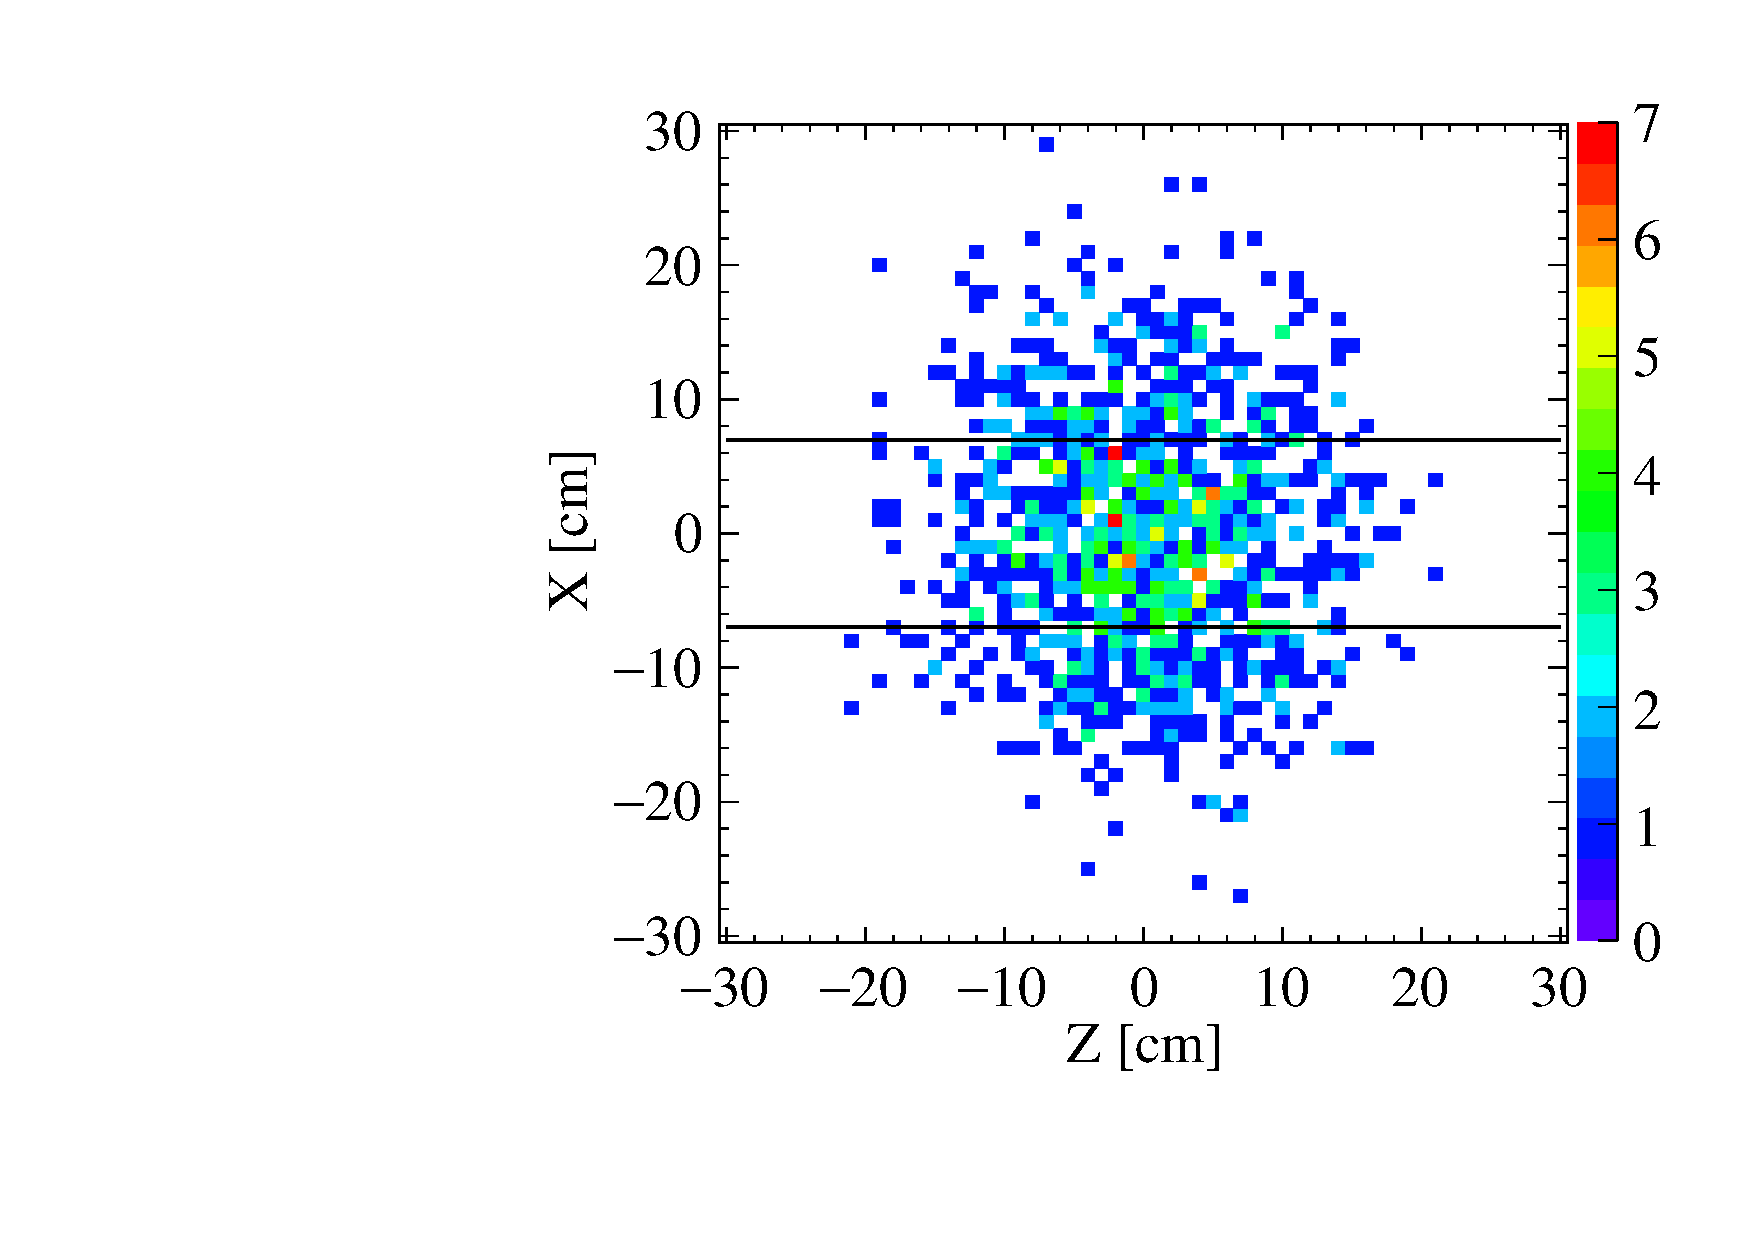
\includegraphics[width=1.0\textwidth]{Chapter8_analysis_jpet/img/3g_xz_all}
  \caption{Side view image}\label{fig:3g_image_b}
\end{subfigure}
\caption{Distribution of the reconstructed origin points of 3$\gamma$ annihilation events identified in the test measurement data. Black lines indicate limits of the 3$\gamma$ production chamber used used in the measurement.}\label{fig:3g_image}
\end{figure}

The statistical limitations of the data sample obtained with the 2-day measurement in absence of an ortho-positronium production medium do not allow for a quantitative estimation of the reconstruction resolution. However, the reconstructed points are grouped in proximity of the geometrical limits of the 3$\gamma$ production chamber, indicated with black lines in~\fref{fig:3g_image}. Moreover, in case of the longitudinal image (\fref{fig:3g_image_b}), the populated region along detector $z$ axis is similar to the $z$ range of efficient 2$\gamma$ imaging (compare~\fref{fig:2g_image_b}), as expected from the considerations presented in the previous Section.

\subsection{Discussion of the results and perspectives}
\label{sec:jpet_discussion_perspectives}

Distributions of reconstructed annihilation points obtained with the test run, in conjunction with the validation of the trilaterative reconstruction method using Monte Carlo simulations show good prospects for future experiments with the \mbox{J-PET} detector with a view to testing the fundamental discrete symmetries.
The present result is limited in terms of statistics, purity of the event sample used and detector resolution. Each of these effects, however, is expected to be improved in the planned measurements.
Once an ortho-positronium production medium is included in the setup, the yield of 3$\gamma$ annihilations will increase by about two orders of magnitude, allowing for easier selection of a pure 3$\gamma$ event sample. The latter will be further aided by the fact that genuine \ops/$\to 3\gamma$ events, as opposed to direct $e^+e^-$ direct annihilations used in this test study, will involve a characteristic time interval between an associated deexcitation photon (corresponding approximately to the \ops/ formation) and recording of the annihilation photons. This property may be used for more sophisticated identification of the ortho-positronium annihilations.

The angular resolution of reconstructed $\gamma$ annihilations points, crucial for control of polarization in the experiment, may be improved by means of a kinematic fit requiring the radial cylindrical coordinate of the reconstruction results to be contained within the annihilation medium as demonstrated using Monte-Carlo simulated events~\cite{gajos_gps}. Moreover, the procedures for calibration and reconstruction of times in the \mbox{J-PET} detector are being improved on at the time of writing of this Thesis, with a view to improving the time resolution which has a deciding impact on the performance of trilateration-based 3$\gamma$ event reconstruction. Advanced signal reconstruction techniques have also been prepared and tested using a \mbox{J-PET} detector prototype~\cite{lech_compressive, neha_synchronized} and their inclusion in the future experiments would provide a further resolution enhancement.


%%% Local Variables:
%%% TeX-master: "../main"
%%% End:
